% by Mirella M. Moro; version: January/18/2012 @ 04:16pm
% -- 01/18/2012: more discussion on SBBD + JIDM; overall revision
% -- 09/03/2010: bib file with names for proceedings and journals; cls with shrinked {received}
% -- 08/27/2010: appendix, table example, more explanation within comments, editors' data

\documentclass[jidm,a4paper]{jidm} % NOTE: JIDM is published on A4 paper
\usepackage{graphicx,url}  % for using figures and url format
\usepackage{epstopdf} 
\usepackage[T1]{fontenc}   % avoids warnings such as "LaTeX Font Warning: Font shape 'OMS/cmtt/m/n' undefined"
\usepackage{amssymb,amsmath}
\usepackage{algorithm}
\usepackage{algorithmic}
\usepackage{listings}

%\usepackage{cite} % NOTE: do **not** include this package because it conflicts with jidm.bst

\graphicspath{{../../images/}}


% Standard definitions
\newtheorem{theorem}{Theorem}[section]
\newtheorem{conjecture}[theorem]{Conjecture}
\newtheorem{corollary}[theorem]{Corollary}
\newtheorem{proposition}[theorem]{Proposition}
\newtheorem{lemma}[theorem]{Lemma}
\newdef{definition}[theorem]{Definition}
\newdef{remark}[theorem]{Remark}

% New environment definition
\newenvironment{latexcode}
{\ttfamily\vspace{0.1in}\setlength{\parindent}{18pt}}
{\vspace{0.1in}}

% ALL FIELDS UNTIL BEGIN{document} ARE MANDATORY

% The following data (volume, number and page) are given by the editors prior to publishing your article
\jidmVolume{3}
\jidmNumber{3}
\jidmYear{12}
\jidmMonth{October}
\setcounter{page}{1}


% Includes headers with simplified name of the authors and article title
\markboth{A. C. S. Furtado}
{CPU consolidation for database workloads in the cloud}
%  -> \markboth{}{}
%         takes 2 arguments
%         ex: \markboth{M. M. Moro}{Any article title}


% Title of the article
\title{CPU consolidation for database workloads in the cloud}


% List of authors
%IF THERE ARE TWO or more institutions, please use:
%\author{Name of Author1\inst{1}, Name of Author2\inst{2}, Name of Author3\inst{2}}
\author{Antonio Carlos S. Furtado}


%Affiliation and email
\institute{Universidade Federal do Parana, Brazil \\ \email{acsfj08@inf.ufpr.br}
% IF THERE IS ANOTHER INSTITUTION:
%\and Name_of_the_second_institution \\
%\email{address@whatever.com}
}


% Article abstract - it should be from 100 to 300 words
\begin{abstract}
Private clouds can be used to consolidate several database management systems. They propitiate a reduction on the cost of ownership by allowing a better utilization of the available resources. The problem is how to split them among the database systems to achieve the best overall performance. In this article, we focus on one resource, namely CPU. We expose an implementation of a virtualization design advisor. It aims to improve the CPU utilization for multiple database workloads running within a a determined host from a private cloud. This is achieved through the recommendation of  configuration parameters for a group of virtual machines, which contain the database systems.
\end{abstract}


% ACM Computing Classification System categories
\category{H.2.2}{Database Management}{Physical Design} 
\category{H.3}{Information Storage and Retrieval}{Systems and Software -- Distributed Systems}
%\category{I.7}{Document and Text Processing}{Miscellaneous}

% Categories and Descriptors are available at the 1998 ACM Computing Classification System
% http://www.acm.org/about/class/1998/
%  -> \category{}{}{}
%         takes 3 arguments for the Computing Reviews Classification Scheme.
%         ex: \category{D.3.3}{Programming Languages}{Language Constructs and Features}
%                   [data types and structures]
%                   the last argument, in square brackets, is optional.

% Article keywords
\keywords{cloud, resource consolidation}
%  -> \keywords{} (in alphabetical order \keywords{document processing, sequences,
%                      string searching, subsequences, substrings})


% THE ARTICLE BEGINS
\begin{document}

% This is optional:
\begin{bottomstuff}
% similar to \thanks
% for authors' addresses; research/grant statements
\end{bottomstuff}

\maketitle


% ARTICLE NEW SECTION
\section{Introduction}

\label{Introduction}

Private clouds are aimed to give local users an agile and flexible infrastructure to run service workloads in their administrative domains. These users are offered virtual machines (VMs), which are scheduled in a group of physical machines within their organization, which we call a cluster. This leads to a better utilization of resources, since services with little demand can be packed into the same machine, process known as server consolidation. This means that on private clouds there is the possibility to cut IT costs, since the consolidation aims to minimize the number of physical servers needed. Other benefits, such as the migration of VMs between hosts and the ability to dynamically change the 
amount of resources provided to it, enabled by technology present in virtual machine monitors (VMMs), make it 
possible to deal with fluctuations in the workload. These characteristics propitiate an elastic environment, which is good for a private cloud, and vital for the pay-on-demand model used in public clouds.  

\subsection{Context}

A cloud is highly dependable on machine virtualization, essential to achieve its goals. Database management systems (DBMSes), like other software systems, are also increasingly being run on virtualized environments for many reasons. Some of them are mentioned in \cite{4498282}, \cite{4401021} and \cite{Soror:2008:AVM:1376616.1376711}, which include the reduction on the cost of ownership, better provisioning and manageability of applications and the ability to migrate them among physical hosts. Our article is motivated by the possibility to take a variety of databases that run on dedicated computing resources and move them to a shared resource pool, on a private cloud, process known as \textit{Database Consolidation}. This scenario is discussed in \cite{instance1290}, in which it is given a good example of how consolidation is applied in a production environment. It lists two deployment models in which this process may be performed onto a private cloud. 

In our article, the deployment model considered is the \textit{Infrastructure Cloud} model, illustrated in figure  ~\ref{fig:infra-model}. In this model, there is generally a one-to-many relationship between servers and VM guests, considered by this article. When a database service is requested, the whole operating system stack is built and provided. Elasticity in this model is limited. Although VM guests may be provided more virtual resources ( CPU or Memory ), they cannot span across servers ( i.e. they are limited to the resources from the server they are running on ). This means that the full resources of the private cloud cannot be brought to bear on a workload requirement. However, the guests will be able to benefit from the live migration feature, supported by most hypervisors, and thus be moved to a host with more resource availability. 

\begin{figure}[t]
\centering
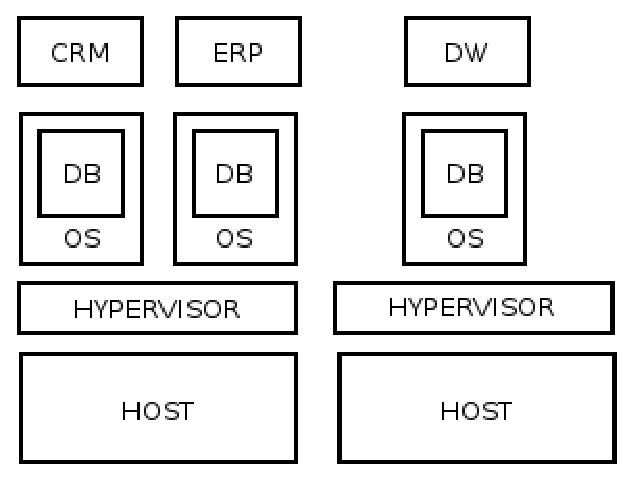
\includegraphics[width=0.3\textwidth]{infra-model.eps}
\caption{Infrastructure cloud deployment model}
\label{fig:infra-model}
\end{figure} 

Some considerations should be made before adopting this deployment model. First, the virtualization will not reduce the number of DBMSes and operating systems, which will surely result in an overhead. It also will not probably be as high performing as other existing non-virtualized alternatives, as I/O intensive workloads may not perform as well in virtualized environments. However, it provides high fault and resource isolation, straightforward database deployment via VM templates and  support for multiple DBMS versions and configurations.


\subsection{Objective}

The problem addressed by our article is formalized in \cite{4401021}, which defined it as the \textit{Virtualization Design Problem} (i.e. resource consolidation problem ) for relational database workloads. It can be defined as follows: \textit{"Given N database workloads that will run on N database systems inside N virtual 
machines, how should we allocate the available resources to these N virtual machines to get the best overall performance?"}. According to the mentioned paper, this problem may find a better solution when applied to relational database systems due to three factors. First, relational database workloads consist of SQL queries with constrained and highly specialized resource usage patterns. Second , queries are highly variable in the way they use resources -- one query might heavily need CPU, while another might need I/O bandwidth instead. Thus, they could benefit from the dynamism in resource allocation. Third, database systems already have a way of modelling their own performance, namely the query optimizer.

As mentioned, DBMSes have particularities involving their workloads. Therefore, the application running inside a VM should not be treated as a black box. Instead, the database system cost model should be exploited. As VMMs have parameters to control the share of physical resources, database systems also have tuning parameters to manage their own performance. These two sets need to be simultaneously analyzed and tuned. In \cite{Soror:2008:AVM:1376616.1376711}, this is a principle of its proposed \textit{virtualization design advisor}. It works by recommending configuration parameters for a group of VMs, each one containing a DBMS. These parameters determine how the shared resources will be allocated to each VM, and consequently to each DBMS. It uses information about anticipated workloads to specify these parameters offline. Furthermore, runtime information collected after the deployment of the recommended configuration can be used to refine this recommendation and to handle fluctuations in the workload. However, this advisor was not originally created to be run on a cloud, rather it has been implemented and tested on a single physical machine, in which two DBMS instances were deployed.

This article serves to describe our implementation of the virtualization design advisor in a cloud environment. Our objective is to solve the \textit{Virtualization Design Problem} in a distributed manner. For each host in a private cloud, we create a corresponding instance of our advisor. Each instance will optimize the CPU among several database workloads. This differs form the scenario considered in \cite{Soror:2008:AVM:1376616.1376711}. Instead of deploying the virtual machines on a single server, we consider a private cloud in our scenario. However, the way our advisor works does not differ from the original because hosts inside a private cloud don't share resources. Other difference is that our implementation focus only on CPU because  generally the query optimization performed by DBMSes is highly sensitive to this resource. They often have one or more tuning parameters used to describe it. By improving the reallocation of the CPU, we expect significant changes in the plans and execution times of the queries. The support of multiple resource types is left for future work. In \cite{Storm:2006:ASM:1182635.1164220} and \cite{springerlink:10.1007/3-540-44469-6_9}, the dynamic reallocation of other resources is discussed. \cite{Soror:2008:AVM:1376616.1376711} also gives an overview on how to model the cost variation of multiple resources.


%Even though in \cite{Soror:2008:AVM:1376616.1376711} the advisor is said to support multiple resource types, this paper is restricted to the consolidation of CPU.

Because of the modular architecture of the advisor proposed in \cite{Soror:2008:AVM:1376616.1376711}, our implementation follows the same approach and splits the advisor into several classes. It is responsible for running and analyzing the database workloads  at the same time. First, it gives each one of them a certain CPU allocation, according to estimates. While a workload is being run, it corrects for any estimation errors and also detects changes in the workload ( i.e. whether it is becoming more or less CPU intensive ). This implementation was developed to work along a virtual infrastructure manager, namely OpenNebula, responsible for managing the private cloud. This integration has a lot of benefits. First, it makes it easier to obtain information about cloud objects, including virtual machines, hosts, etc. Our advisor can also make use of scripts and features already included in this manager. Furthermore, we are able to integrate any other third-party solution build for OpenNebula with our advisor. In this article, we detail how we were able to integrate our advisor to this manager. In addition, we comment OpenNebula's limitations, and how they were overcome in order to develop our solution.

%In this implementation, our focus is to optimize the CPU allocation among database workloads. However, our idea is that this could be expanded in a future work, in order to support multiple resource types. Therefore, in this article our objective is not to show a final and complete solution to the virtualization design problem. Here we introduce this problem and we show that just by reallocating one resource, we can improve the performance of running database workloads in a cloud. 

The rest of this article is structured as follows. Chapter ~\ref{chap:relwork} is used to discuss related work, including the description of the \textit{virtualization design advisor}. Chapter ~\ref{chap:infrastructure} is used to show how a cloud infrastructure is managed. In section ~\ref{chap:implementation}, we show how the integration of the advisor within the cloud management system was implemented. Chapter ~\ref{chap:results} is used to show the results obtained. Finally, section ~\ref{chap:final} presents some final considerations and ideas for future work.


\section{Related Work}

\label{chap:relwork}


In \cite{dias:automatic}, some considerations are made on how to compare CPU capacity in distributed systems. It also explains how changes in the CPU capacity affect the database. Regarding CPU virtualization, \cite{6127969} contains a study on its overhead. It provides a system to measure it and performs some experiments using as the Xen\footnote{http://xen.org} as the hypervisor. It shows that the overhead increases proportionally to the number of virtual machine guests deployed in a determined host. However, the CPU utilisation is improved, since reduces idle time. 

\cite{Soror:2008:AVM:1376616.1376711-OLD} shows how CPU costs should be modelled. It explains the process of building these cost models through information obtained from the DBMS and a way to dynamically schedule the CPU among the database workloads. \cite{Soror:2008:AVM:1376616.1376711-OLD} evolved to \cite{Soror:2008:AVM:1376616.1376711}, which is more detailed and discusses how multiple resources are scheduled. The latter serves as base for our article, since it describes the virtualization design advisor, which will be detailed in the following section.


\subsection{Virtualization design advisor}

\label{chap:virtualization}


In \cite{Soror:2008:AVM:1376616.1376711}, the author considers a typical resource consolidation scenario, in which several DBMS instances, each one of them running in a separate VM, share a common pool of physical resources. As discussed earlier, this article addresses the problem of optimizing the performance of these instances by controlling some configuration parameters of the VM guests. These parameters determine how the resources should be indirectly allocated to each DBMS instance. This scenario is illustrated in ~\ref{fig:scenario}.


\begin{figure}[t]
\centering
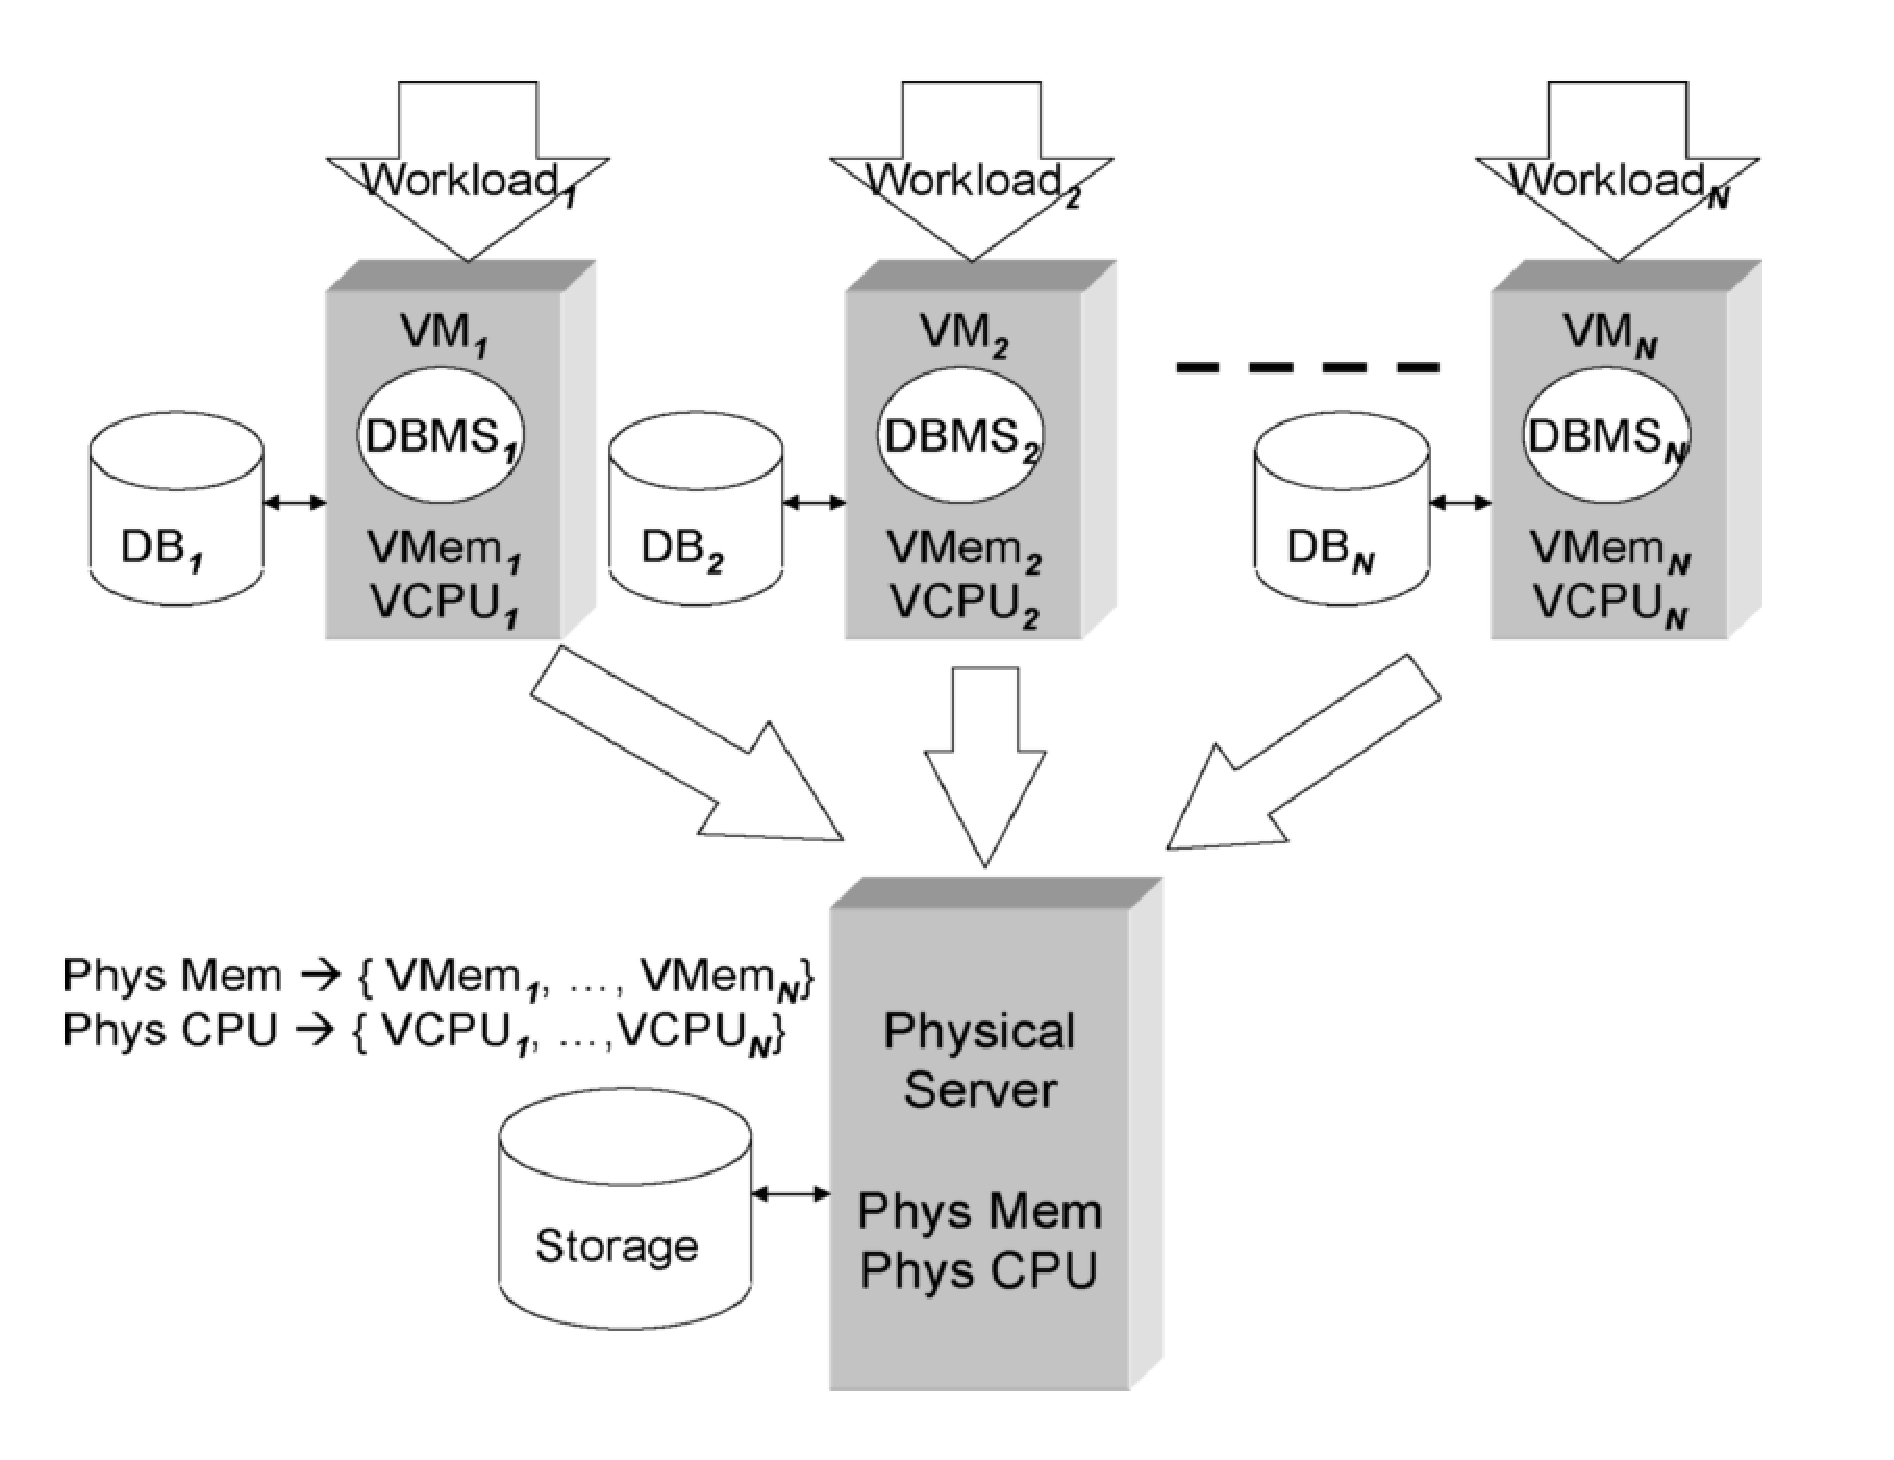
\includegraphics[width=0.4\textwidth]{dbms_consolidation.eps}
\caption{Resource Consolidation scenario}
\label{fig:scenario}
\end{figure} 

\subsection{Problem definition}

In order to model this problem, the author assumes that there are  $M$ types of resources, such as CPU capacity, memory, or I/O bandwidth. The notation used to represent the share of resources allocated to a VM running a workload $W_{i}$ is $R_{i} = [r_{i1},...r_{iM}], 0 \leq r_{ij} \leq 1$. It is also considered that each workload $W_{i}$ has the same monitoring interval for all the VMs ( i.e. the workloads represent the statements processed by different DBMS instances in the same amount of time ).

Each workload is associated to a cost, which depends on the resource share allocated to the VM in which it runs. The notation $Cost(W_{i},R_{i})$ is used to represent the cost of running the workload $W_{i}$ under resource allocation $R_{i}$. Considering that there are $N$ workloads, the goal is to choose $r_{ij}, 1 \leq i \leq N, 1 \leq j \leq M$ such that the following formula is minimized:
\[
  \sum_{i=1}^{N} Cost(W_{i},R_{i})
\].

This problem was generalized to satisfy Quality of Service (QoS) requirements. One of these requirements is the possibility to specify the maximum increase in cost that is allowed for a workload under the recommended resource allocation. In order to model this requirement, it was defined a \textit{cost degradation} as
\[
 Degradation(W_{i},R_{i}) = \frac{Cost(W_{i},R_{i})}{Cost(W_{i},[1,...,1])}
\]
, where $[1,...,1]$ represents the resource allocation in which all of the available resources are allocated to $W_{i}$. It can be specified a \textit{degradation limit} $L_{i} ( L_{i} \geq 1 )$, such that 
\[
 Degradation(W_{i}, R_{i}) \leq L_{i}
\]
for all $i$. This limit is set per workload, so it does not need information about other workloads that it will be sharing the physical server with.

Other QoS requirement introduced involves the ability to specify relative priorities among the different workloads. A \textit{benefit gain factor} $G_{i} (G_{i} \geq 1)$ can be used to indicate how important it is to improve the performance of $W_{i}$. Each unit of improvement is considered to worth $G_{i}$ cost units. When this parameter is applied to the problem, it may cause a workload to get more resources than its fair share. In order to incorporate it to our problem, the cost equation is modified to minimize the following
\[
  \sum_{i=1}^{N} G_{i} * Cost(W_{i},R_{i})
\]


\subsection{Architecture}

The process of  determining the allocation of resources to each VM is neither immediate, nor static. The proposed advisor follows a sequence of steps. Initially, it makes a resource allocation based on the workload descriptions and performance goals, which is performed offline ( i.e. the VMs are not running yet ). Then all of the subsequent steps are performed online. It adjusts its recommendations based on the difference between expected and actual workload costs to correct for any cost estimation errors made during the initial phase. At the same time, it uses continuing monitoring information to dynamically detect changes in the workloads. This last step is important because a workload cannot be considered static, its resource needs may change during execution. In both of these online steps, the resource allocation step may occasionally be performed again with updated cost models. This approach prevents the advisor from allocating resources to DBMS instances that will obtain little benefit from them. These 
resources need to be given to the workloads that need them the most.

Since the advisor does not consist of one single task, it makes sense to organize the flow of its tasks. An overview of this advisor in a modular way is given in figure ~\ref{fig:architecture}. This article intends to give a brief explanation of each task.


\begin{figure}[t]
\centering
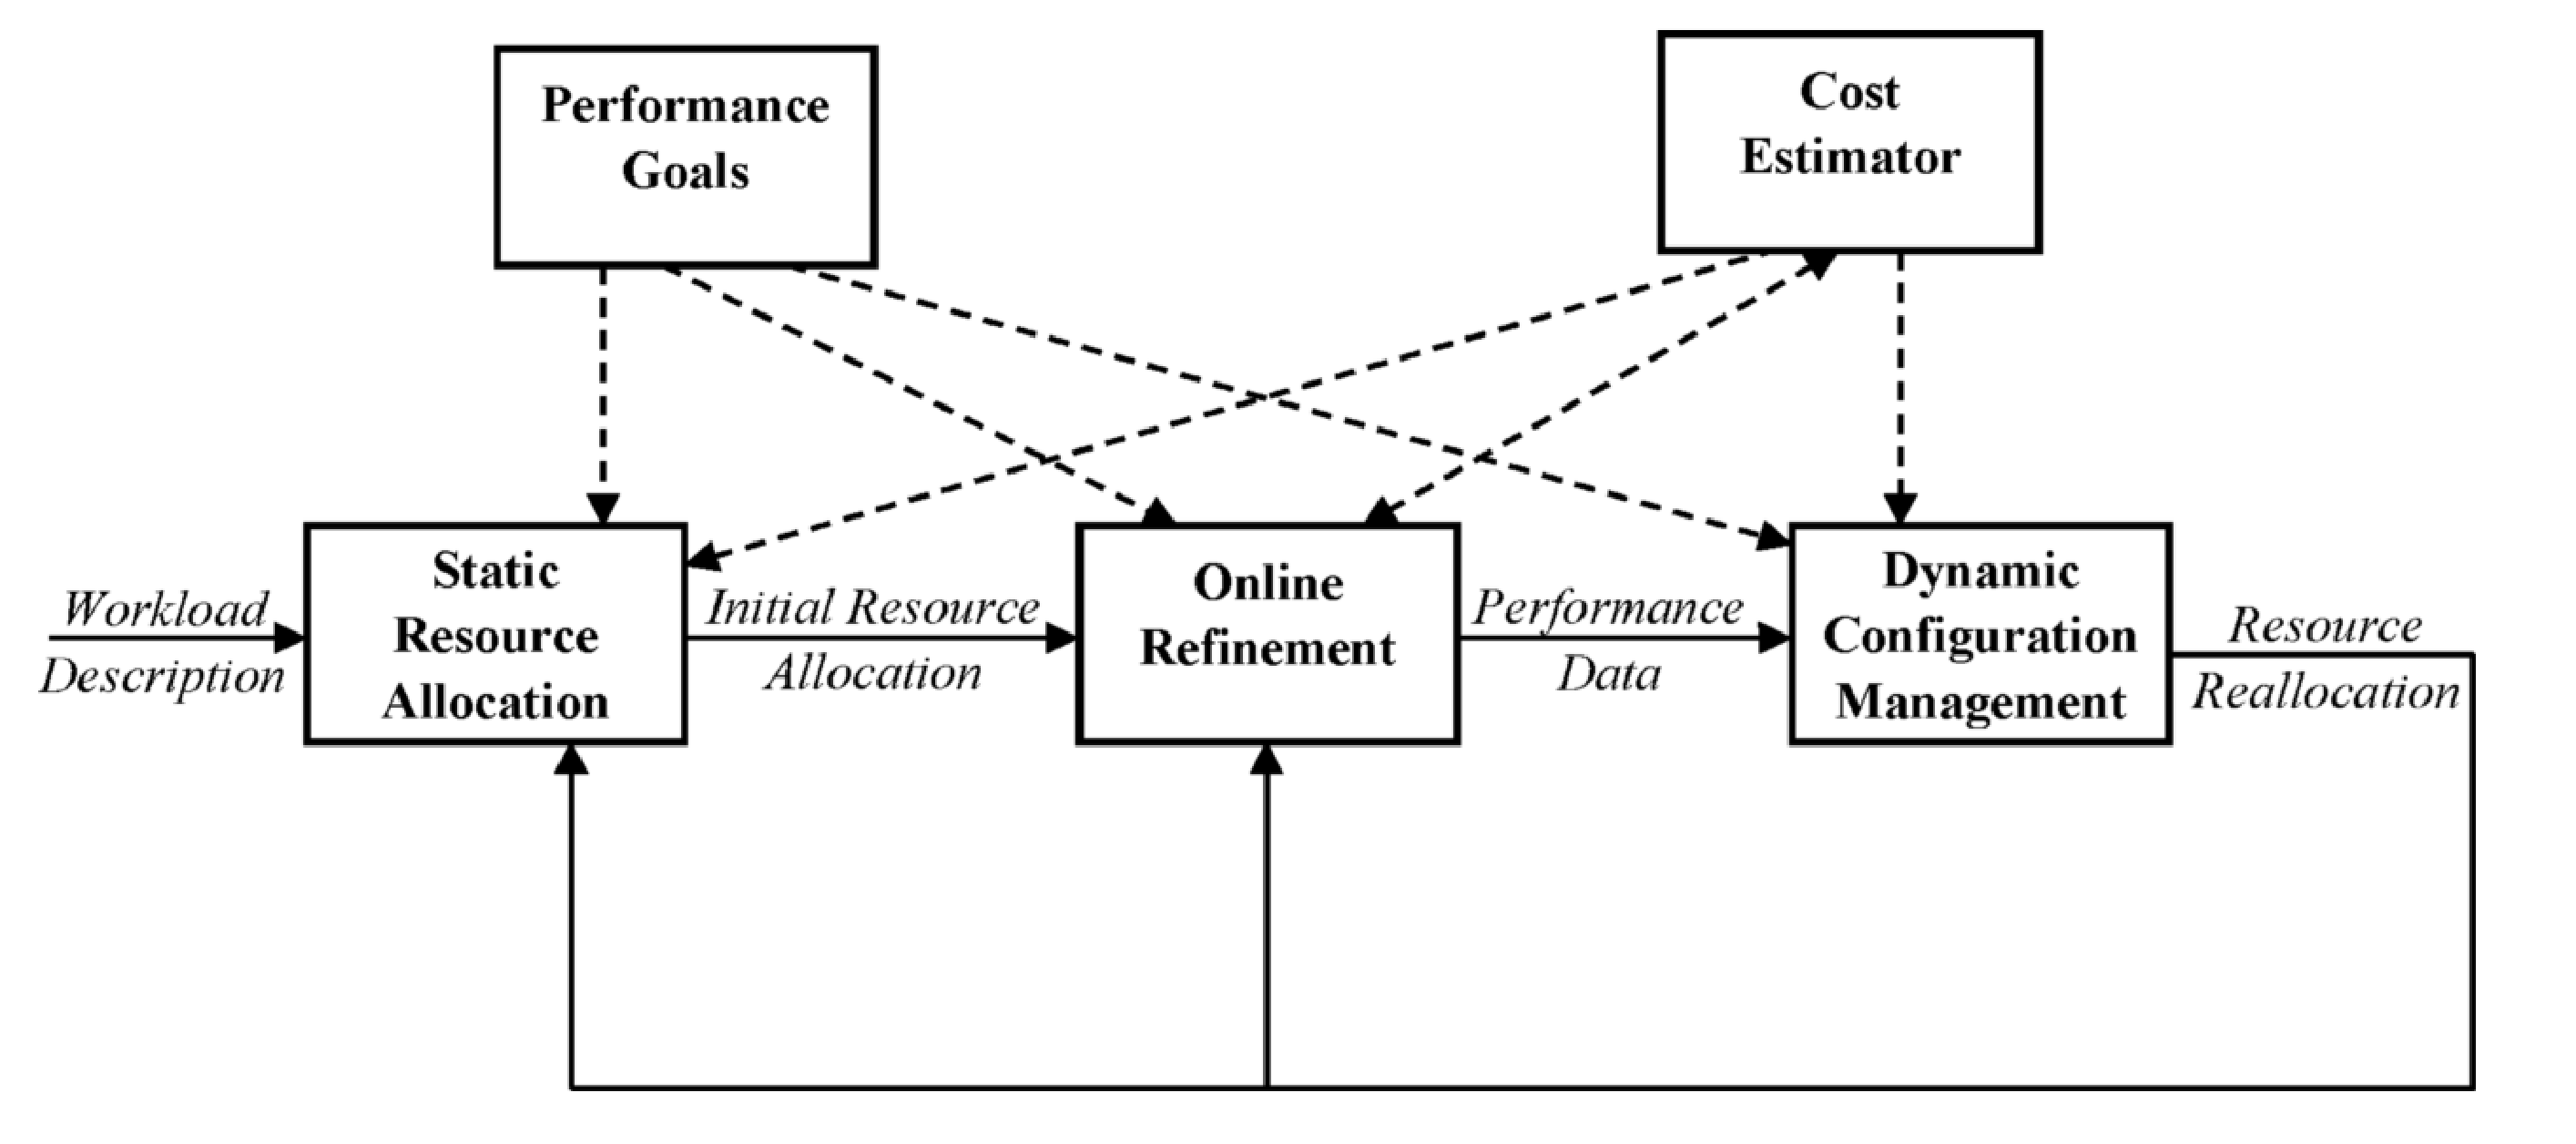
\includegraphics[width=0.5\textwidth]{architecture.eps}
\caption{Advisor overview}
\label{fig:architecture}
\end{figure} 

\subsubsection{Cost estimation and initial allocation}
\label{subsec:cost}

Given a workload $W_{i}$, the cost estimator will predict $Cost(W_{i},R_{i})$. The strategy used to implement this module is to leverage the cost models built into database systems for query optimization. The query optimizer cost model can be described as $Cost_{DB}(W_{i},P_{i},D_{i})$, where $W_{i}$ is a SQL workload, $P_{i} = [p_{i1},..,p_{iL}]$ is a vector of parameters that are used to list both the available computing resources and DBMS configuration parameters relevant to the cost model, and $D_{i}$ is  the database instance. 

The author identifies two problems in using only query optimizer cost models. The first problem is the difficulty of comparing cost estimates produced by different DBMSes. They may have different cost models. Even if they share the same notion of cost, the normalization process may differ. This problem is addressed partially by the advisor. It assumes that the DBMSes have the same notion of cost, and it proposes a renormalization step to make $Cost_{DB}(W_{i},P_{i},D_{i})$ from different DBMSes comparable.% This step is not considered for implementation, since the support of multiple DBMSes is out of the scope of this paper.

The second problem is that the query optimizer cost estimates depends on $P_{i}$, while the virtualization design advisor is given a candidate resource allocation $R_{i}$. The mapping of these two parameters is achieved through a calibration step. This step determines a set of DBMS cost model configuration parameters according to the different possible candidate resource allocations. It is supposed to be performed per DBMS on the physical machine before running the virtualization design advisor. Once the appropriate configuration parameters $P_{i}$ are determined for every possible $R_{i}$, the DBMS cost model is used to generate $Cost_{DB}$.

The calibration step is performed on  \textit{descriptive parameters}, which are used to characterize the execution environment. The approach to the \textit{prescriptive parameters}, which control the configuration of the DBMS itself, is to leave it for user definition. 

%For instance, in ~\ref{table:descritive} it is shown some descriptive parameters used in PostgreSQL, while in ~\ref{table:prescritive} it is shown some prescriptive ones. 


% \begin{table}[t]
% 
%     \caption{Descritive parameters}
%     \label{table:descritive}
%     \sffamily
% 
%     \centering
%     \begin{tabular}{ | l | p{5cm} |}
%     \hline
%     Parameter & Description  \\ \hline
%     \textbf{random\_page\_cost} & Cost of non-sequential page I/O \\ \hline
%     \textbf{cpu\_tuple\_cost} & CPU cost of processing one tuple \\ \hline
%     \textbf{effective\_page\_size} & size of file system's page size  \\
%     \hline
%     \end{tabular}
%     \rmfamily
% 
% \end{table}
% 
% 
% \begin{table}[t]
% 
%     \caption{Prescritive parameters}
%     \label{table:prescritive}
%     \sffamily
% 
%     \centering
%     \begin{tabular}{ | l | p{5cm} |}
%     \hline
%       Parameter & Description  \\ \hline
%     \textbf{shared\_buffers} & shared bufferpool size \\ \hline
%     \textbf{work\_mem} & amount of memory used by each sort and hashing operator. \\
%     \hline
%     \end{tabular}
%     \rmfamily
% 
% 
% \end{table}

The calibration step follows a basic methodology for each parameter $p_{ij} \in P_{i}$, described below:

\begin{itemize}
 \item (1) Define a calibration query $Q$ and a calibration database $D$, such that $Cost_{DB}(Q,P_{i},D)$ is independent for all descritive parameters in $P_{i}$, except for $p_{ij}$; \\
  \item (2) Choose a resource allocation $R_{i}$, instantiate $D$, and run $Q$ under that resource allocation, and measure the execution time $T_{Q}$; \\
%  \item (3) This step refers to the renormalization of the $Cost_{DB}$ provided by the DBMS. As mentioned earlier in this section, we are not going into the details of this step; \\
  \item (3) Perform the renormalization of $Cost_{DB}$ provided by the DBMS, in order to transform it to a common notion of cost; \\
  \item (4) Repeat the two preceding steps for a variety of $R_{i}$ allocations. $r_{ij} \in R_{i}$ only needs to be varied if $p_{ij}$ describes that resource. For instance, query optimizer parameters that describe CPU, I/O and memory are independent of each other and can be calibrated independently. This should avoid unnecessary calculations; \\
  \item (5) Perform regression analysis on the set of $(R_{i},p_{ij})$ value pairs to determine a calibration function $Cal_{ij}$ that maps resource allocations to $p_{ij}$ values. \\
\end{itemize}

During the described methodology, calibration queries should be carefully chosen. They need to be dependent only on the parameter that is being calibrated. If it is not possible to isolate one parameter, a system of $k$ equations is solved to determine the values for the $k$ parameters.

After the calibration is performed, the advisor is ready to be run. First, it needs to provide an initial configuration.  \cite{Soror:2008:AVM:1376616.1376711} proposes a greedy search to find an optimal allocation among the VM guests. The algorithm starts by assigning a $\frac{1}{N}$ share of each resource to each one of the $N$ workloads. Then it iteratively considers shifting a small amount of resources from one workload to another. It tries to obtain the maximum benefit from adjusting each resource. The search is performed until no more optimizations are possible.


%From experimental results, the creator of this algorithm observed that the greedy search is very often optimal and always within $5\%$ of the optimal allocation. This result is a good indicative for the algorithm, as it tells us that it hardly gets stuck in local minimums.



\subsubsection{Online refinement}
\label{subsec:ref}

The initial allocation is based on the calibrated query optimizer cost model, as described earlier. This enables the advisor to make recommendations based on an informed cost model. However, this model may have inaccuracies that lead to sub-optimal recommendations. The  \textit{online refinement} is based on the observation of the actual times of execution for a workload. It uses these observations to refine resource allocation recommendations. Then the advisor is rerun with the new cost models, so  we can obtain an improved resource allocation for different workloads. These optimizations are performed until the allocations stabilize (i.e. the new recommendation is equal to the last one ). It is important to notice that the goal of the \textit{online refinement} is not to deal with dynamic changes in the workload, which are dealt by another module, but to correct cost models. Thus, it is assumed that the workload is not going to change during this process. 

In order to optimize the recommendations, it is necessary to identify the cost model behaviour. The author identifies two types of models. The first is the \textit{linear model}, which can describe, among other resources, the allocation of CPU. For this resource, workload completion times are linear in the inverse of the resource allocation level. Therefore, the cost model in this case can be represented by
\[
 Cost(W_{i}, [r_{i}]) = \frac{\alpha_{i}}{r_{i}} +\beta_{i}.
\]

The values $\alpha_{i}$ and $\beta_{i}$ are obtained through a linear regression. This regression is performed on multiple points that represent estimated costs for different $r_{i}$ values used during the initial allocation phase. This cost is adjusted by two parameters, $Est_{i}$ and $Act_{i}$. They represent the estimated cost for workload $W_{i}$ and the runtime cost, respectively. When the cost is underestimated, these parameters are used to increase the slope of our cost equation. From another standpoint, when this value is overestimated, we need to decrease the slope. This is achieved by refining the cost through the equation
\[
  Cost'(W_{i}, [r_{i}]) = \frac{Act_{i}}{Est_{i}} * \frac{\alpha_{i}}{r_{i}} + \frac{Act_{i}}{Est_{i}} * \beta_{i}.
\]

However, not all resources are linear. The second type of cost model identified is the \textit{piecewise-linear}, which describes, among others, the allocation of memory. Increasing this resource does not consistently result in performance gain. The magnitude and the rate of improvement change according to the query execution plan. The cost equation is similar to the linear cost model, and it is given by
\[
  Cost'(W_{i}, [r_{i}]) = \frac{Act_{i}}{Est_{i}} * \frac{\alpha_{ij}}{r_{i}} + \frac{Act_{i}}{Est_{i}} * \beta_{ij}, r_{i} \in A_{ij}.
\]
The difference here is the parameter $A_{ij}$, which represents the interval of resource allocation levels corresponding to a particular query execution plan, represented by $j$. Its intervals are obtained during the initial phase, when the query optimizer is called with different resource allocations and returns different query execution plans with their respective costs. These query execution plans define the boundaries of the $A_{ij}$ intervals. The end of this interval is the largest resource allocation level for which the query optimizer produced this plan. The initial values of $\alpha_{ij}$ and $\beta_{ij}$ are obtained through linear regression. Together with $A_{ij}$, they are subsequently adjusted.

Both the equations presented work within their cost model. Nevertheless, a physical  machine has more than one type of resource. Therefore, the author extends the cost equations to multiple resources. In this extension, it is considered that $M$ resources are recommended, such that $M-1$ resources can be modelled using a linear function, while the resource $M$ is modelled using a piecewise-linear function. The cost of workload $W_{i}$, given a resource allocation $R_{i} = [r_{i1},...,r_{iM}]$ can be given by
\[
  Cost'(W_{i}, R_{i}) = \sum_{j=1}^{M} \frac{Act_{i}}{Est_{i}} * \frac{\alpha_{ijk}}{r_{ij}} + \frac{Act_{i}}{Est_{i}} * \beta_{ik}, r_{iM} \in A_{iMk},
\]
in which $k$ represents a certain query execution plan, which defines the boundaries of $A_{iMk}$. 

During refinement, this equation is supposed to be performed iteratively, in order to optimize the parameters $\alpha_{ijk}$ and $\beta_{ijk}$. This iteration is shown below.
\begin{eqnarray*}
 Cost'(W_{i}, R_{i}) &=& \sum_{j=1}^{M} \frac{Act_{i}}{Est_{i}} * \frac{\alpha_{ijk}}{r_{ij}} + \frac{Act_{i}}{Est_{i}} * \beta_{ik} = \sum_{j=1}^{M} \frac{\alpha'_{ijk}}{r_{ij}} + \beta'_{ik}, r_{iM} \in A_{iMk} \\
 Cost''(W_{i}, R_{i}) &=& \sum_{j=1}^{M} \frac{Act_{i}}{Est_{i}} * \frac{\alpha'_{ijk}}{r_{ij}} + \frac{Act_{i}}{Est_{i}} * \beta'_{ik} = \sum_{j=1}^{M} \frac{\alpha''_{ijk}}{r_{ij}} + \beta''_{ik}, r_{iM} \in A_{iMk} \\
  &\vdots&
\end{eqnarray*}

The author in \cite{Soror:2008:AVM:1376616.1376711} proposes a heuristic that changes the equation in the first iteration. Instead of  considering the interval $A_{iMk}$, the first iteration scales to all the intervals of the cost equation (i.e., for all $k$). This is done because the estimation errors can be partly due to a bias in the query optimizer's view of resource allocation levels. In the second iteration and beyond, this cost will be refined according to the interval $A_{iMk}$, where the resource $r_{iM}$ will be scaled.

%These refinement iterations stop when the refinement continues beyond $M$ iterations. In this case the refinement process continues, but through a linear regression model to the observed points. At this point, the query optimizer's estimates are just dropped. This process only finishes when the number of iterations reach an upper bound, placed manually. It is used to guarantee termination.

After refining the cost equations, the advisor is rerun. If the newly obtained resource allocation is the same as the original, the refinement process is stopped. Otherwise, it goes on.

\subsubsection{Dynamic configuration management}

\label{subsec:dcm}
Even if we have an optimal resource allocation, the workload may change its behaviour during execution. It may occur due to the intensity of the workload (e.g. increased number of clients), or the nature of the workload (e.g. new set of queries with different resource needs ). These changes are not dealt by the online refinement process, that is why the dynamic configuration management is needed. 

The proposed approach consists in monitoring the relative changes in the average cost per query between periods. If the change in the estimated query is above a threshold, $\theta$, we classify this a major change. When this situation is identified, it is decided to make the virtualization design advisor restart its cost modelling from scratch, before online refinement. The cost model needs to be discarded, since it no longer reflects information about the workload.

In order to deal with minor changes, it is introduced a new metric $E_{ip}$. It represents the relative error between the estimated and the observed cost of running workload $W_{i}$ in monitoring period $p$. We analyse two consecutive periods. If both $E_{i(p-1)}$ and $E_{ip}$ are below some threshold ( e.g. $5\%$ ), or if $E_{ip} - E_{i(p-1)} > 0$, then we continue with online refinement. In this case, the errors are either small, or are decreasing. Both of these situations can be efficiently dealt by some iterations of online refinement. However, if this condition is not satisfied, the cost model is discarded once again. 

\section{Cloud infrastructure management}
\label{chap:infrastructure}

This section will be used to describe OpenNebula, the virtual infrastructure (VI) manager chosen to have the virtualization design advisor implemented over. Organizations can use it to manage and deploy VMs, individually or in groups that must be co-scheduled on local or external resources. It merges a lot of different technologies, in order to allow users to design their private or hybrid clouds. Some of its key features are:
\begin{itemize}
 \item It provides a homogeneous view of resources, regardless of the underlying hypervisor (e.g. KVM, Xen, etc.). This makes the virtualization much less restrictive. The physical machine in which the VM is being run does not need to be tied to a specific virtualization technology, which may cause incompatibility issues;
  \item It manages a VM full life cycle, it is used to specify storage requirements and setting up the network;
  \item Supports configurable resource allocation policies.
\end{itemize}

The OpenNebula architecture is illustrated in figure ~\ref{fig:open_arch}. It can basically be split into three layers. The core (middle layer ), which has three management areas. One of them is dealing with the creation of virtual networks, which is done through the Virtual Network (VN) manager. This component is responsible for handing out and keeping track of leases ( composed by one IP and one MAC address valid on a particular network ), and their associations with VMs and physical bridges used. Second, it needs to manage and monitor the physical hosts, which is the responsibility of the host manager. And finally, there is the VM manager, responsible for taking care of a VM's life cycle. It prepares the disk images for them, by controlling the image and storage technologies. It also needs to control the hypervisors, responsible for their creation and control. And combined with the VN manager, this manager provides the VM with the network environment. Another important feature in the core is achieved with 
the SQL Pool. It is responsible for saving the OpenNebula state. Even after a shutdown or a failure, it is possible to restore a previous state. All the managers make use of this Pool to store information.


\begin{figure}[t]
  \centering
 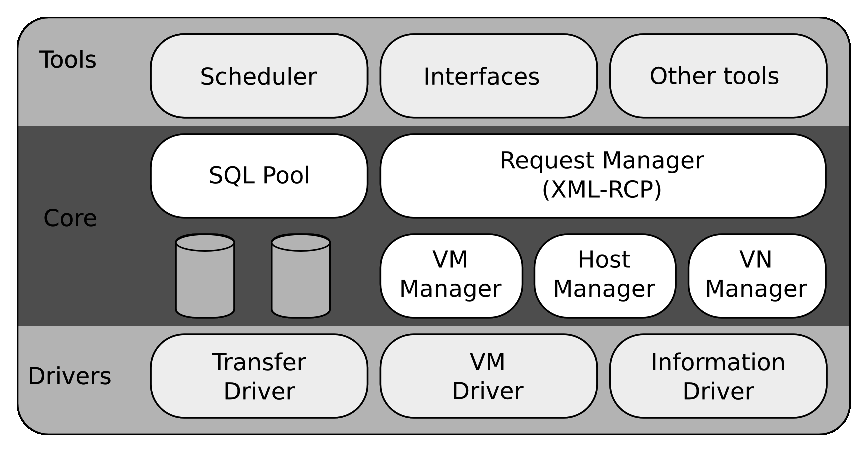
\includegraphics[width=0.5\textwidth]{one-architecture_2.eps}
  \caption{OpenNebula architecture}
  \label{fig:open_arch}
\end{figure}

One important feature of the core module is the service deployment support. The Request manager exposes a XML-RPC interface that decouples most of the functionality present in the core. Through this interface it is possible to control and manage any OpenNebula resource, including virtual machines, networks, images, hosts, etc. As OpenNebula is in continuing development, it is expected that this API will support even more functionality. Currently, it is known that dynamic resource allocation is not supported yet. All the resource allocation is performed offline, through VM templates. The amount of resources allocated is passed from the templates directly to the hypervisors, and they will be the same until the end of that VM's life cycle. We will discuss more about this issue on the next section, as resource reallocation is important for the advisor.

All these described activities are performed through pluggable drivers, present in the bottom layer. This modularity makes the system easier to extend and avoids tying it to any specific technology. The drivers shown in figure ~\ref{fig:open_arch}  address some particular areas, such as virtualization ( by communicating with the hypervisor ), storage operations, gather monitoring information and authenticate user requests.

Other way of extending OpenNebula is through hooks, controlled by the Hook manager. They enable the triggering of custom scripts tied to a change in a particular resource, being that a Host or a Virtual Machine. This opens a wide area of automation for system administrators. Below is an example of a hook, namely "error", defined in the proper configuration file. It is used to perform recovery actions when a host fails ( i.e. it enters in the ERROR state ). When this happens, the script host\_error.rb is called with the host id passed as an argument. The "remote" parameter tells that this script should be executed in the OpenNebula server, and not in the failed host. The purpose of this script is to resubmit all the VMs that were running on the failed host, for them to be run on active hosts. 

\begin{itemize}
 \item HOST\_HOOK $=$ [ \\
    name      $=$ "error",\\
    on        $=$ "ERROR",\\
    command   $=$ "host\_error.rb",\\
    arguments $=$ "\$HID",\\
    remote    $=$ no ]\\
\end{itemize}

In the top layer there are user interfaces to access OpenNebula, and also APIs extended from the XML-RPC interface, which can work between the core and other tools. One of these APIs is  OCA\footnote{OpenNebula Cloud API}. It exposes the same functionality as XML-RPC, in a more convenient way. Other relevant module for this article is the OpenNebula's scheduler, also in the top layer. Its job is to make placement decisions for the VMs ( i.e. it assigns physical machines for VMs ). It has access to all requests OpenNebula receives. Based on these requests, it keeps track on allocations and sends the appropriate deployment commands to OpenNebula's core. As other modules, it can be replaced by third party solutions, such as Haizea\footnote{http://haizea.cs.uchicago.edu/},  which offers more sophisticated placement policies. However, in this article we will stick to the OpenNebula's default scheduler. Next, we will describe it in more details.

\subsection{Scheduler}

The scheduler already present in OpenNebula works only with immediate provisioning. Its concept is pretty straightforward, the resources are only provisioned at the moment they are required, if that is not possible, then the requirement is ignored. The requirements are done in a manual and static way, in which the amount of resources, among other configurations, are defined in a file. The assignment is performed through a classification policy.  The administrator needs to set a \textit{RANK} variable, which defines which host is more suitable for a VM. Each VM has its own \textit{RANK} equation, and the scheduler assigns a host with the highest value for this variable to a VM. In OpenNebula, deployments are performed through VM templates, so you can share the same scheduling policy  to a group of VMs. For instance, here are some possible \textit{RANK} definitions, each one serving a specific policy:

\begin{itemize}
 \item Load-aware Policy
 \begin{itemize}
   \item \textbf{Heuristic:} Use nodes with less load;
   \item \textbf{Implementation:} Use nodes with more \textit{FREECPU} first.
    \item \textit{RANK} = \textit{FREECPU}

 \end{itemize}

  \item Striping policy
  \begin{itemize}
   \item \textbf{Heuristic:} Spread the VMs in the cluster node;
   \item \textbf{Implementation:} Use the nodes with less VMs running first.
   \item \textit{RANK} = "\textit{- RUNNING\_VMS}"
  \end{itemize}

\end{itemize}

Furthermore, users may use the same syntax applied to \textit{RANK} statements to define a \textit{REQUIREMENT}. Requirements are used to set placement constraints. They rule out hosts from the list of machines suitable to run a certain VM. Below is an example of a requirement statement. It only allows  a VM to be run by nodes with CPUs that have clock higher than $1000 MHz$:
\begin{itemize}
 \item \textit{REQUIREMENT} = \textit{CPUSPEED} $> 1000$ 
\end{itemize}



\section{Implementation}

\label{chap:implementation}

In this section, it is discussed the virtualization design advisor implementation over OpenNebula. Our aim is to optimize the distribution of CPU inside a private cloud for VM guests running database workloads. However, in order to make this work feasible, some restrictions were made. They will be explained as the advisor is detailed.

For organizational purposes and better integration with OpenNebula, our solution  is part of a module called OpenRC, which stands for Open Resource Consolidation. It was designed to work alongside OCA, since it will need full access to OpenNebula functionality. As OCA, it was also implemented in Ruby\footnote{http://www.ruby-lang.org} language. In this module, it was implemented both the steps presented in figure ~\ref{fig:architecture}, from section ~\ref{chap:virtualization}, and missing features from OpenNebula, needed for the advisor.

One of the missing features in OpenNebula is the ability to dynamically reallocate resources, as mentioned in section ~\ref{chap:infrastructure}. Although it is not supported by OpenNebula, most hypervisors currently support it for some types of resource. Besides the need for changes in the OpenNebula drivers to support these operations, it would be necessary to extend the OpenNebula's core to handle them. Instead, it was decided to implement this functionality in OpenRC, with information provided by OCA. The approach to achieve this  was the use of libvirt\footnote{http://libvirt.org/}, which defines itself as "A toolkit to interact with the virtualization capabilities of recent versions of Linux (and other OSes)". It offers an API that works with all the hypervisors supported by OpenNebula, offering many features, including CPU limitation. Currently, OpenNebula already has a libvirt API, which enables VM management over the core layer. OpenRC uses libvirt at a lower level, correspondent to OpenNebula's 
bottom layer. Libvirt currently has three parameters that allows us to control the CPU scheduling. Here is an explanation of their use:
\begin{itemize}
 \item \textbf{quota} and \textbf{period}: These parameters work together, they allow us to set a hard limit for the cpu usage. \textbf{Period} should be in range $[1000, 1000000]$. Within it, each virtual CPU of the VM will not allowed to consume more than \textbf{quota} worth of runtime. For instance, the following values define that the VM guest will be limited to $20\%$ of CPU time:
  \begin{itemize}
   \item  \textbf{period}$=100000$; 
   \item \textbf{quota}$=20000$;
  \end{itemize}
  \item \textbf{shares}: Opposite to the previous parameters, \textbf{shares} enables us to set a soft limit for CPU usage. It specifies the proportional weighted share for the VM guest. Its value is relative. For instance, a VM configured with value $2048$ will get twice as much CPU time as a VM with value $1024$. However, if the CPU is not being used by the VM with a higher parameter value, the other will not be denied CPU idle time.
\end{itemize}

These parameters are indirectly updated and retrieved through a class called \textbf{CPULimitation}, within OpenRC. The objective of this class is to set hard/soft limits for CPU usage of OpenNebula VMs on remote hosts. Our approach to execute these remote commands  is the same as OpenNebula, in fact for this task we only import the OpenNebula's class \textbf{RemotesCommand}, which is responsible for executing OpenNebula commands through Secure Shell (SSH) on remote hosts.

Other implemented feature was the communication with the DBMS running inside the VM guest. This was achieved by the creation of the \textbf{DatabaseHelper} class. Structured according to the facade pattern, it enables access to a set of classes, responsible for establishing a database connection, set tuning parameters, process single queries or workloads, obtain estimated and actual runtime costs, etc. This pattern was chosen to make the support of other DBMSes easier in future work. For the purposes of this article, only PostgreSQL\footnote{http://www.postgresql.org/} was supported and tested as DBMS. This decision was not only based on implementation details, but also to ease cost modeling and parameter calibration. The support of a new DBMS starts by the creation of a module, representing the DBMS. In this module,  it should be defined classes which have its functionality exposed by \textbf{DatabaseHelper}, as illustrated by figure ~\ref{fig:facade}. As these classes have database specific methods, 
they should not be 
directly implemented in the facade object. For instance, when a query is run for analyzing purposes, the costs are not obtained the same way for different DBMS types. Once the database module is created, following specific implementation rules, it can be easily included. 

\begin{figure}[t]
  \centering
 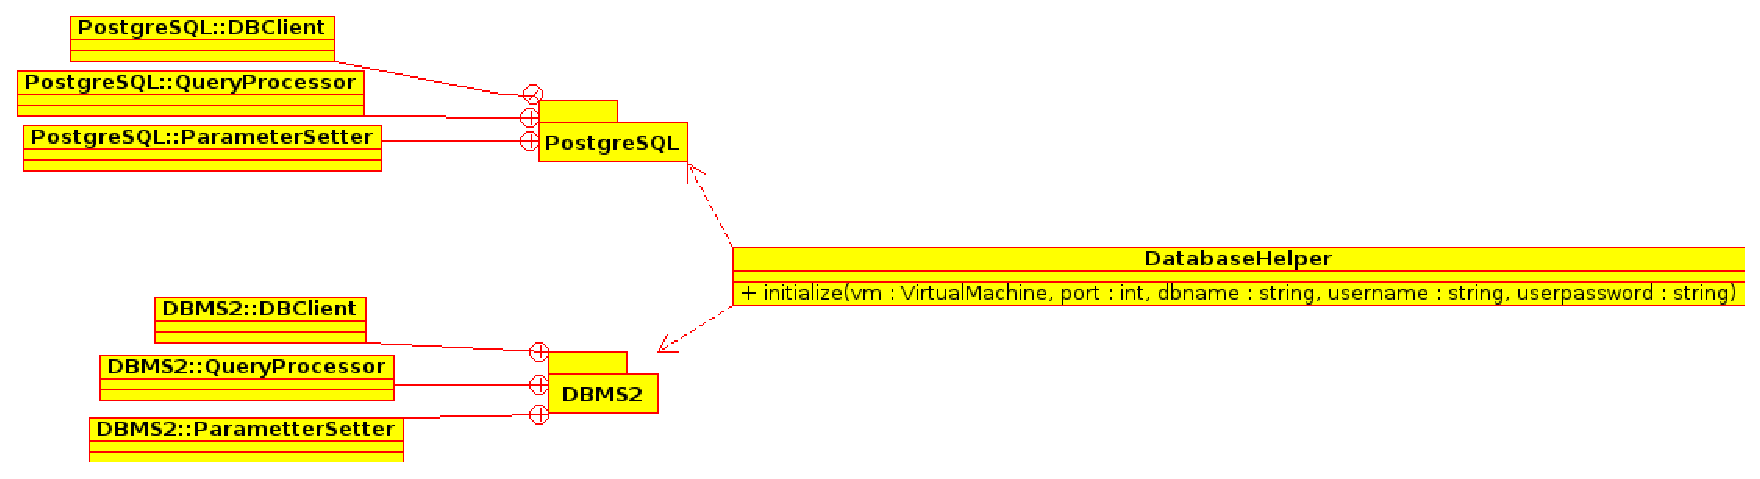
\includegraphics[scale=0.5]{database_helper_facade.eps}
  \caption{DatabaseHelper facade with an eventual support of a second DBMS}
  \label{fig:facade}
\end{figure}

A \textbf{DatabaseHelper} instance needs to be initialized with a \textbf{VirtualMachine} object, defined in OCA. As mentioned in section ~\ref{chap:infrastructure}, OpenNebula is able to define both the MAC and IP addresses of a Virtual Machine, in form of a lease. It also keeps track of these leases in its SQL Pool. As any other pool element, this information can be retrieved through OCA, in XML format. So when a VM is passed to our class, it is possible to retrieve the IP address of that VM and connect to PostgreSQL. As some authentication parameters ( database name, user name, user password ) are also needed for database connection, and they are not stored by OpenNebula SQL pool, they must be passed manually to our solution.

As soon as the communication with the DBMS and the CPU limitation were implemented, it was possible to start developing modules inherent to our advisor. In the following subsections, every part of the process has its implementation detailed.

\subsection{Calibration}
\label{sec:calib}

The first step in order to implement the advisor is the creation of a calibration process. As discussed earlier, this task is responsible for mapping the query optimizer's cost model, which depends on its parameters $P_{i}$, to  the advisor's cost model, based on resources $R_{i}$. Without it, it is not possible to build a proper cost estimator. Since the calibration should be performed before any VM deployment on each physical host on our cloud, it was decided that this process should become an OpenNebula hook. The hook definition is given below:
\begin{itemize}
 \item HOST\_HOOK $=$ [ \\
    name      $=$ "Calibration",\\
    on        $=$ "CREATE",\\
    command   $=$ "openrc/host\_db\_calibration.rb",\\
    arguments $=$ "\$HID",\\
    remote    $=$ no ]\\
\end{itemize}

This hook will execute the host\_db\_calibration.rb script on the OpenNebula server whenever a new host is created, passing the host id as argument. In this script, the whole calibration process is performed, as described in section ~\ref{chap:virtualization}. Initially, it searches for the image of a specific VM, which basically contains the calibration database. As hosts and virtual machines, images are also objects managed by OpenNebula. Thus, it needs to be added to the image pool before running the calibration script.

The calibration database running inside the VM is generated by pgbench\footnote{http://www.postgresql.org/docs/devel/static/pgbench.html}. This tool is able to run benchmark tests, based on TPC-B, for PostgreSQL. During implementation, it was only used to generate and populate our calibration database. Its choice relies on its integration with PostgreSQL, usability, and the ability to populate databases with custom sizes.

Once the calibration database is up and running, it is necessary to run specially designed queries to find out the relation between different resource allocation levels and tuning parameters costs.  As mentioned in subsection ~\ref{subsec:cost}, DBMSes generally do not  share the same notion of cost. It means that we must also find the relation between DBMS estimated costs and actual costs, which would be the execution times. In PostgreSQL, all costs are normalized with the respect of time required for a single page to be fetched from disk. This cost is represented by the parameter $seq\_page\_cost$. Therefore, by finding its actual value, we also find this relation. 


Our approach to find the actual cost values for $seq\_page\_cost$ was to use a tool to find the virtual disk throughput. In this implementation, the tool hdparm\footnote{http://sourceforge.net/projects/hdparm/} was chosen. Among other features, this utility serves as a disk benchmarking alternative for Linux. It must be previously installed in the calibration VM. Its results are obtained through a specially designed PostgreSQL function, added to the calibration database. Based on the results retrieved from this function, the cost of $seq\_page\_cost$ is calculated. Besides this calculation, it is also important to decide how to simulate I/O disk contention at this step. This would happen in production environments, where multiples VM guests are run concurrently. Calculating $seq\_page\_cost$ without considering a realistic scenario could lead to inaccurate results. It was decided to magnify this problem by stressing the host disk while the costs are being generated and retrieved. The stress\footnote{
http://freecode.com/projects/stress} utility was chosen to generate disk stress. It is used to spin several 
workers writing on files and removing directory entries on the remote host. In a more realistic setup, the VMs would compete less for I/0, and probably this cost would have a certain variability. By stressing the disk, our aim is to simulate a worst-case scenario. 


After finding the relation between the DBMS estimated cost and the actual cost ( i.e. execution time ), it is possible to calibrate the tuning parameters. Since this article is restricted to reallocate CPU among VMs, only parameters that describe CPU need to be calibrated. For PostgreSQL, these parameters are shown below.

\begin{table}[t]
    \centering
    \caption{Parameters that describe CPU}
    \label{table:descriptive}
    \sffamily


    \begin{tabular}{ | l | p{5cm} |}
    \hline
    Parameter & Description  \\ \hline
    \textbf{cpu\_operator\_cost} & Cost of processing each operator or function call \\ \hline
    \textbf{cpu\_tuple\_cost} & Cost of processing one tuple (row) \\ \hline
    \textbf{cpu\_index\_tuple\_cost} & Cost of processing each index entry during an index scan  \\
    \hline
    \end{tabular}
    \rmfamily

\end{table}


PostgreSQL uses these parameters to build its query optimizer's cost estimates. That is why a lot of documentation can be found on how to tune these parameters in order to obtain better cost execution plans. However, the way these parameters are exactly used within these plans is poorly documented. Only by observing the source code is possible to determine how they are applied to simple query plans. The first two parameters at table ~\ref{table:descriptive}, $cpu\_tuple\_cost$ and $cpu\_operator\_cost$ can be obtained by the query presented at subsection ~\ref{app:cal1}. Without changing the values of any PostgreSQL's default parameter values, this query will always have the same execution plan generated. It will access the table $pgbench\_accounts$ using a sequential scan, and subsequently perform an aggregation. PostgreSQL has the following equations for these two operations:
\begin{equation}
  \begin{split}
      SEQSCAN &= ( seq\_page\_cost * num\; pages \; fetched ) + ( cpu\_tuple\_cost * number\; rows ) \\
      AGGREGATE &= SEQSCAN + ( cpu\_operator\_cost * number\; rows) \\
  \end{split}
\end{equation}

The estimated cost and execution times for these equations can be obtained by executing this query on PostgreSQL with the command $EXPLAIN (ANALYZE)$. In this case, the query will actually be run and an execution plan will be returned. Each step in the execution plan has its corresponding costs indicated. This means that it is possible to isolate costs for each operation from the total. Based on the actual costs returned, our script is able to deduct the parameters from the equations. However, by retrieving these costs we get a different scale, as the actual costs are in milliseconds, instead of page fetches. We use the actual value of $seq\_page\_cost$ to make conversions between different scales. The equation is given below:
\[
 param_{estimated} = \frac{param_{actual}}{seq\_page\_cost_{actual}}
\]

To calculate the first two descriptive parameters, only one modification to the original equation was made. During a $SEQSCAN$, PostgreSQL accounts for the cost of fetching pages from disk. The problem is to determine how many pages were actually fetched. One approach would be running the query with the command $EXPLAIN (ANALYZE,BUFFERS)$. By using this command, it is informed the number of pages hit in the PostgreSQL cache and number of pages that needed to be read. However, the PostgreSQL cache may not reflect the state of the operating system cache. During experimentations, changes in the hit/miss ratio did not incur in an expected change in actual costs. Our approach was to cache all the data for the consults and limit the number of page accesses of a determined query. After doing that, costs related to disk page fetches were ignored from the equation.

The third descriptive parameter, $cpu\_index\_tuple\_cost$ , is used during index scans. It can be obtained through the query presented in subsection ~\ref{app:cal1}. Before running this query, it is necessary to set the following parameters:
\begin{eqnarray*}
 enable\_seqscan&=&off \\
 enable\_bitmapscan&=&off \\
\end{eqnarray*}
This will force the planner to use an index scan plan, as $aid$ is a primary key, instead of a sequential scan. Its equation is much more complex than the previous one. Mainly because it involves a lot of I/O cost estimates. In addition to $seq\_page\_cost$, its plan is highly dependable on another parameter, namely $random\_page\_cost$. It represents the cost of fetching a non-sequentially disk page. During estimation, PostgreSQL uses an approximation of pages actually fetched after accounting for cache effects. This approximation is proposed in \cite{Mackert:1989:ISU:68012.68016}. The number of fetched pages is

\begin{eqnarray*}
  PF=&& \\
  &min(2TNs/(2T+Ns),T)\qquad \qquad \qquad & when\quad T \le b \\
  &2TNs/(2T+Ns) & when \quad (T > b) \wedge (Ns \le 2Tb/(2T-b)) \\
  &b + (Ns -2Tb/(2T-b))*(T-b)/T & when \quad (T > b) \wedge (Ns > 2Tb/(2T-b)) \\
\end{eqnarray*}
where
\begin{description}
 \item T $=$ number of pages in table;
 \item N $=$ number of tuples in table;
 \item s $=$ selectivity $=$ fraction of table to be scanned;
 \item b $=$ number of buffer pages available.
\end{description}

For the same reasons why I/O cost was discarded for the first equation, we decided to eliminate it from the $cpu\_index\_tuple\_cost$ calculation. Since we are only interested in CPU cost, instead of I/0, we cache all the data to be retrieved and consider the following parameters to be
\begin{equation}
 \begin{split}
  seq\_page\_cost &= 0 \\
  random\_page\_cost &= 0
 \end{split}
\end{equation}

Given this configuration, the equation for a single index scan can be defined as
\begin{eqnarray*}
  \lefteqn{Cost=} \\
  &&ntuples * ( cpu\_index\_tuple\_cost + qual\_op ) + \\
  &&100*cpu\_operator\_cost + \\
  &&cpu\_per\_tuple\_cost * ntuples + ( I/0\;Cost ) \\
  \lefteqn{qual\_op=} \\
  &&cpu\_operator\_cost * ncond \\
  \lefteqn{cpu\_per\_tuple\_cost=} \\
  &&cpu\_tuple\_cost + cpu\_operator\_cost * nfilters
\end{eqnarray*}
,where
\begin{description}
 \item ntuples $=$ number of tuples retrieved;
 \item ncond $=$ number of index conditions;
 \item nfilters $=$ number of filters ( including index conditions );
 \item I/O cost $=$ indicates the cost of fetching pages from disk, related to parameters $seq\_page\_cost$ and $random\_page\_cost$. As it is discarded by the calibration process, it will not be detailed.
\end{description}

The values for $cpu\_tuple\_cost$ and $cpu\_operator\_cost$ and the details about our calibration query and database are already known. As we discared the I/O cost from our equation, there is only one variable left to be deducted, that is $cpu\_index\_tuple\_cost$. The calibration process then isolates this variable from the rest of the equation and finds its value under different resource allocations, like it was done for the two first parameters. The library built to enable CPU limitation is used here to set a hard limit for CPU usage.

The execution costs found during the calibration step are then stored in files, with the corresponding CPU allocation levels. The collected data is used later by the virtualization design advisor. The process shown here in this section is database specific, as it is necessary previous knowledge about the DBMS cost model. One point to consider is that the support of new DBMSes can be much harder. If a DBMS does not offer tools for self calibration, its descriptive parameters must be calibrated manually, as seen in this section. This requires an investigation on how these parameters are used internally to build query plans.

\subsection{Virtualization Design Advisor}

After the end of the calibration process for a certain host, the virtualization design advisor can start handling database workloads and resource allocation levels. The advisor modules, shown in figure ~\ref{fig:architecture}, served as a base on how to organize our implementation. This can be seen on figure ~\ref{fig:advisor}. Here, a new process was added, namely \textbf{LoadGenerator}.  Its task is to run the workloads under resource allocations conditions established during \textbf{ConfigurationSearch}. The costs obtained through execution are passed to both \textbf{OnlineRefinement} and \textbf{DynamicConfigurationManagement}. During workload execution, this class may call \textbf{ConfigurationSearch} several times for reallocation, regarding changes in the workload or recurrent allocation optimizations. In this section, each class within the advisor will be detailed.


\begin{figure}[ht]
\centering
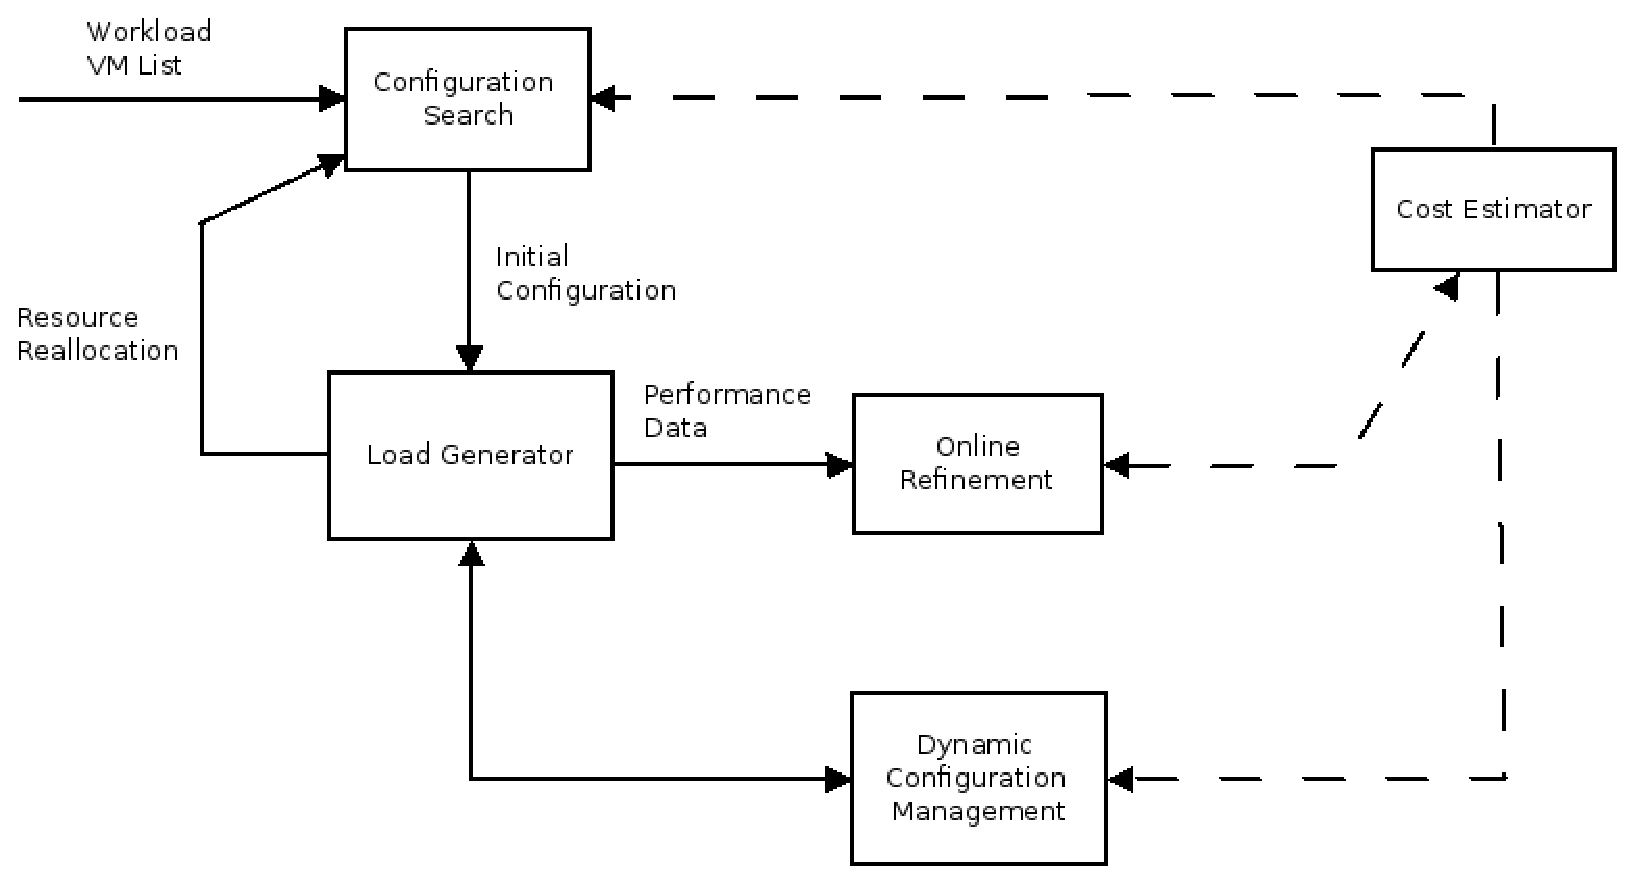
\includegraphics[width=0.6\textwidth]{advisor-arch.eps}
\caption{Implementation overview}
\label{fig:advisor}
\end{figure} 

\subsubsection{Configuration Search}

The \textbf{ConfigurationSearch} class, from which the advisor is started,  aims to search for an optimal CPU allocation among the VM guests ( i.e. minimize the costs of running the database workloads ). Opposed to \cite{Soror:2008:AVM:1376616.1376711}, we decided not to implement a greedy search for this task . Since we are only reallocating CPU, and its variation is linear, this kind of search is not necessary. The implemented algorithm is shown in section ~\ref{sec:cpusearch}. It considers that the equation of the cost model is represented by the following linear equation:
\[
 Cost(W_{i}, r_{i}) = \frac{\alpha_{i}}{r_{i}} +\beta_{i}.
\].
Therefore, this algorithm is used when CPU, or other resource that varies linearly, is the only one to be reallocated. It works by deducing the value of $\alpha_{i}$ for each workload $W_{i}$. This parameter represents the slope of the cost equation ( i.e. it shows how much our cost improves by increasing $r_{i}$ ). We compare the  value of $\alpha_{i}$ to the slopes of all the workloads. This relative value of $\alpha_{i}$ is used to set the allocation level. For instance, consider the situation in which there are two workloads being run, and one of them improves twice as much as the other one, when added the same amount of resources. In this case, the workload that has a better improvement rate will get two times more CPU as the other one. This means that we are not interested in the cost itself, but how much it benefits from CPU adjustment. One benefit from this algorithm, when compared to the greedy search, is that it makes less calls to the DBMS query optimizer cost estimator. It does not need to iteratively shift an amount of resources from one workload to another.


Other characteristic of this class is that it is the only one that actually changes the resource allocation levels. Considering that a private cloud is composed of multiple hosts, it is necessary to run multiple instances of this class. It was created a daemon to manage these multiple searches. It waits for virtual machines to be started and also for workloads to be run on these VMs. Then it resends this information to the \textbf{ConfigurationSearch} instance that corresponds to the host in which that particular VM was designated to be run. Information about newly created VMs can be automatically added as soon as they are created, through an OpenNebula hook. On the other hand, workloads are sent with a script, which sends their information through a TCP Socket, in an expected format.

The search is used in three occasions. The first is when the advisor is started. The objective, in this case, is to find a better initial allocation than the default ( i.e. find an allocation of resources for the $N$ VM guests better than the proportion $\frac{1}{N}$ ). It relies on estimates provided by the \textbf{CostEstimator} class to accomplish it. In a production environment, a good approach would be to base these estimates in a workload history. As we only have a testing scenario, it was opted to base our search on the first workload that is yet to be run.

In the other two occasions, the search is called by the \textbf{LoadGenerator} class. The first is related to the online refinement process, described in subsection ~\ref{subsec:ref}. As the cost estimator model is refined after each workload execution, new calls are made to reflect these refinement changes in the resource allocation. In this case, the searches are not restarted from the default allocation, instead we search for improvements to the current allocation. If the allocation remains the same after the refinement, this search may not be called any longer by the \textbf{LoadGenerator}. This option can be set by the user. And finally, the last occasion happens when a workload change is detected. Then \textbf{LoadGenerator} calls this class, and the search will be started from scratch. This case is similar to the first search, as both of them start from the default allocation and the cost model is restarted.

Independently on how the search is called, it always ends by applying the resource allocation levels found. \textbf{ConfigurationSearch} is the only class within the advisor that actually changes them. This is applied in two steps. The first corresponds to setting a soft limit on the CPU level for each VM, according to the resource allocation levels found during search. The second step is to set the parameters for each DBMS, also according to the search. After they are applied, the rest of the workload can be run.

\subsubsection{Cost Estimator}

The cost estimation process is performed by the class \textbf{CostEstimator}. The description of how this task should be performed in the virtualization design advisor is given in subsection ~\ref{subsec:cost}. Basically, it needs to provide an estimated cost for running a certain workload under a determined resource allocation level. During initial calls to this estimator, the cost model is not built yet. So \textbf{CostEstimator} leaves this task to be performed by the cost estimator built inside the DBMS query optimizer. Here we face a problem described previously, while our cost model depends on a resource allocation $R_{i}$, the query optimizer cost estimates depend on a set of tuning parameters $P_{i}$. This mapping has already been performed in the calibration process. Therefore, this class collects all calibration data for the tuning parameters and uses linear regression on the observed points. 

The equations obtained through linear regression for each parameter will be used to map $R_{i}$ to $P_{i}$. Besides being useful to the \textbf{CostEstimator} class, they also help the \textbf{ConfigurationSearch} class to know how to set the DMBS parameters under a certain resource allocation level. They stop being used for cost estimation purposes when the cost model is built. Our approach to build the cost model is to keep statistics of previous calls to this class. During an initial search, \textbf{CostEstimator} may be called several times for different resource allocation levels, and so the estimated results are stored. Before running the workload, a linear regression is performed on these points. As in \cite{Soror:2008:AVM:1376616.1376711} CPU is described as a resource that varies linearly, a linear regression model provides a good approximation. After building the cost model, this class stops calling PostgreSQL for estimates. This significantly reduces the extra calls to the DBMS. So the advisor is 
expected to have a better performance as it is being run.

Other difference between our cost estimator and the one built inside the query optimizer is the scale used. Our approach was to use use costs based on query runtime. The reason is that this is easy to determine and a better approach to compare different DBMSes. As already mentioned in section ~\ref{sec:calib}, PostgreSQL has a different notion of cost. Like it was done during the calibration process, we simply use the actual value of $seq\_page\_cost$ to convert between the two scales. Our renormalization equation is the following:
\[
 Cost(W_{i}, r_{i}) = Cost_{DB}(W_{i},P_{i},D_{i}) * seq\_page\_cost_{actual}
\]

. Once the cost model is built, it can be refined by the \textbf{OnlineRefinement} class.

\subsubsection{Online Refinement}

The online refinement process adopted in our advisor is straightforward. Considering that the CPU has a linear model and that we only need to refine this resource, the \textbf{OnlineRefinement} class  is an implementation of the first refinement equation presented in subsection ~\ref{subsec:ref}. This equation is designed specifically for refining resources with linear variation. During execution, the cost model is refined the following way:
\begin{equation}
 \begin{split}
   Cost(W_{i}, r_{i}) & = \frac{\alpha_{i}}{r_{i}} +\beta_{i} \\
   Cost'(W_{i}, r_{i}) & = \frac{Act_{i}}{Est_{i}} * \frac{\alpha_{i}}{r_{i}} + \frac{Act_{i}}{Est_{i}} * \beta_{i} = \frac{\alpha_{i}'}{r_{i}} +\beta_{i}' \\
   Cost''(W_{i}, r_{i}) & = \frac{Act_{i}}{Est_{i}} * \frac{\alpha_{i}'}{r_{i}} + \frac{Act_{i}}{Est_{i}} * \beta_{i}' = \frac{\alpha_{i}''}{r_{i}} +\beta_{i}'' \\
    & \vdots
 \end{split}
\end{equation}

 . $\alpha_{i}$ and $\beta_{i}$ are parameters of the linear model for workload $W_{i}$, and $Act_{i}$ and $Est_{i}$ are the actual and estimated costs for running this workload, respectively. In order to apply these equations, this class needs to receive the estimated and the actual costs for this workload. The actual runtime costs are provided by the \textbf{LoadGenerator} class, and the estimated costs come from the \textbf{CostEstimator}. The latter will have then its cost model updated through the refinement performed.

\subsubsection{Load Generator and Dynamic Configuration Management}

The \textbf{LoadGenerator} class was added to the advisor with the objective to simply run the workloads. Besides increasing the cohesion among the advisor classes, it helps us to determine which parts of the advisor we want to enable. Initial configuration search, online refinement process and the workload change detection may be disabled in order to test a specific scenario in the advisor.

This class launches a thread for each VM running on a certain host, in order to run the workloads concurrently. Each VM is designated a workload queue. Even though workload units may be received from multiple clients, they are stored in a single queue, which is processed sequentially. This definitely differentiates our tests from a production environment, where a database may receive multiple queries concurrently. It limits our advisor in testing workload intensities. Therefore, in this article our results are focused on the workload nature, rather than its intensity. As the execution results are obtained, they are passed to \textbf{OnlineRefinement}, if it is enabled. 

While the \textbf{LoadGenerator} runs the queries for each workload, the \textbf{DynamicConfigurationManagement} monitors this execution periodically. 
It is a simplified version of the module described in subsection ~\ref{subsec:dcm}. Every monitoring period, it checks for relative changes in the cost per query. If the change is above a threshold $\theta$ ( i.e. it is a major change ), it reports it. Otherwise, the changes are ignored.

The relation between these two classes was implemented according to the observer pattern. \textbf{LoadGenerator} acts as the observer, although it only starts observing the class after all the cost models have been defined. If a major change in the workload is detected by \textbf{DynamicConfigurationManagement}, it notifies the observer . When this happens, the \textbf{LoadGenerator} class decides to restart from the greedy search process, discarding the cost model.

One of the virtualization design advisor  features that was left out in this implementation was the support of QoS parameters. This means that during execution, all the workloads are treated equally, and no restrictions are made to their improvement or decrease in performance. The implementation of the \textit{benefitial gain factor} and the \textit{cost degradation} will be left for future work.

\section{Results}

\label{chap:results}

The experiments were conducted using the PostgreSQL 9.0.7 as the database system. Because of the nature of the advisor, all tests were performed on a single host from a cluster managed by OpenNebula 3.6. The host has one 2.4GHz dual core processor and 4GB RAM, running Fedora Linux 16, using kernel version 3.3.8. Even though the the library created to reallocate CPU in OpenRC should work with all the hypervisors supported by Libvirt, the experiments were only performed with KVM\footnote{http://www.linux-kvm.org/}. This hypervisor is already integrated within the mainline Linux kernel since the 2.6.0 kernel version. It was designed to support only hardware assisted virtualization.

For the tests performed during the calibration step, a special VM was created to be run on newly added hosts. It runs the Debian Squeeze Linux operating system, specially configured to be a database server. It contains a simple $300MB$ database, created with PGBench. Changes in the relational schema of the database are not very important for this step, as long as the query execution plans are known beforehand. For this reason, we do not need to go into further details on why a specific schema was chosen. Under the tested host, the VM was given both CPU cores and 2GB of RAM. Considering the database size, it was wholly loaded in memory. This decision does not have any impact on the results, since only the parameters that describe CPU should be calibrated, instead of I/O. The memory storage for PostgreSQL was created using standard features provided by the DBMS and Linux operating system. The PostgreSQL init scripts were modified to automatically handle this storage every time the database service is stopped 
or started, including the VM booting. As the calibration queries have a simple known query plan, the tuning parameters are only modified if their change has an effect on the query optimizer decisions.

All the other tests were performed using Transaction Processing Benchmark H (TPC-H) databases with scale factor $0.6$. When loaded into PostgreSQL with their indexes, the size of these databases is $4339 MB$.  The choice of this benchmark relies on the fact that \cite{Soror:2008:AVM:1376616.1376711} has a previous study on the nature of determined queries from this benchmark. We use this knowledge to create workloads with specific CPU needs during the experiments.  It was also decided that in order to minimize I/O effects, the databases should also be loaded  in a RAM based file system, even though they will not fit entirely in the available memory. Each database runs in a VM with $1.8 GB$ of RAM.  Each virtual machine is assigned one virtual CPU, during the tests they are pinned to the same core. This magnifies the problem of CPU competition among VM guests, especially in our case, where the workloads are sequentially run. 

The sections included in this section follow a sequence similar to the one used in section ~\ref{chap:implementation}. They are used to show experiments used to test different parts of our solution. We start by showing results for the calibration phase, as it needs to be run before the advisor, in order to map resource allocation levels to tuning parameters. Then we show the results related to the execution of our advisor. The first experiment is conducted using static workloads ( i.e. workloads that do not have its CPU needs changed along execution ). It is used to test how effective is the configuration search from OpenRC. In the second experiment, small changes in the workload needs are performed to test how the online refinement step adjusts the cost model during execution. We finish with a third experiment, used to test the dynamic configuration management. Its objective is to observe how the advisor behaves to major changes in the workload.


\subsection{Calibration}

The parameters \textbf{cpu\_tuple\_cost} and \textbf{cpu\_operator\_cost} were calibrated using the query shown in subsection ~\ref{app:cal1}. The values obtained for different resource allocations are shown in figures ~\ref{fig:cpuop} and ~\ref{fig:cputp}, along with the linear regression performed on them. \cite{Soror:2008:AVM:1376616.1376711} has argued that these parameters vary linearly with $1/$(Allocated CPU fraction) because they describe a resource that has a linear variation. However, the figures show that this variation is not strictly linear. Considering the linear equation to be
\[
 f(x) = m*x + b
\],
the asymptotic errors found were the following:
\begin{itemize}
 \item \textbf{cpu\_tuple\_cost}
 \begin{itemize}
  \item $m \approx 6,7\% $;
  \item $b \approx 3,9\% $;
 \end{itemize}
  \item \textbf{cpu\_operator\_cost}
 \begin{itemize}
  \item $m \approx 9.2\% $;
  \item $b \approx 5.6\% $.
 \end{itemize}
\end{itemize}

These errors were observed because of a high deterioration on the performance of the virtualized database for low CPU configurations ( below $30\%$ ). This deterioration also can be seen on \cite{4401021}, even though no explanations are given about why it happens. In \cite{Soror:2008:AVM:1376616.1376711} this situation was not tested, or it was omitted, as it does not show values for the tuning parameters below  a $30\%$ CPU allocation. Further studies could point out how low limits on the CPU capacity affect the performance of virtualized databases. They could also show whether there is a safe limit for CPU allocation, in order to avoid higher deteriorations. 

 
 \begin{figure}[t]
 \centering
 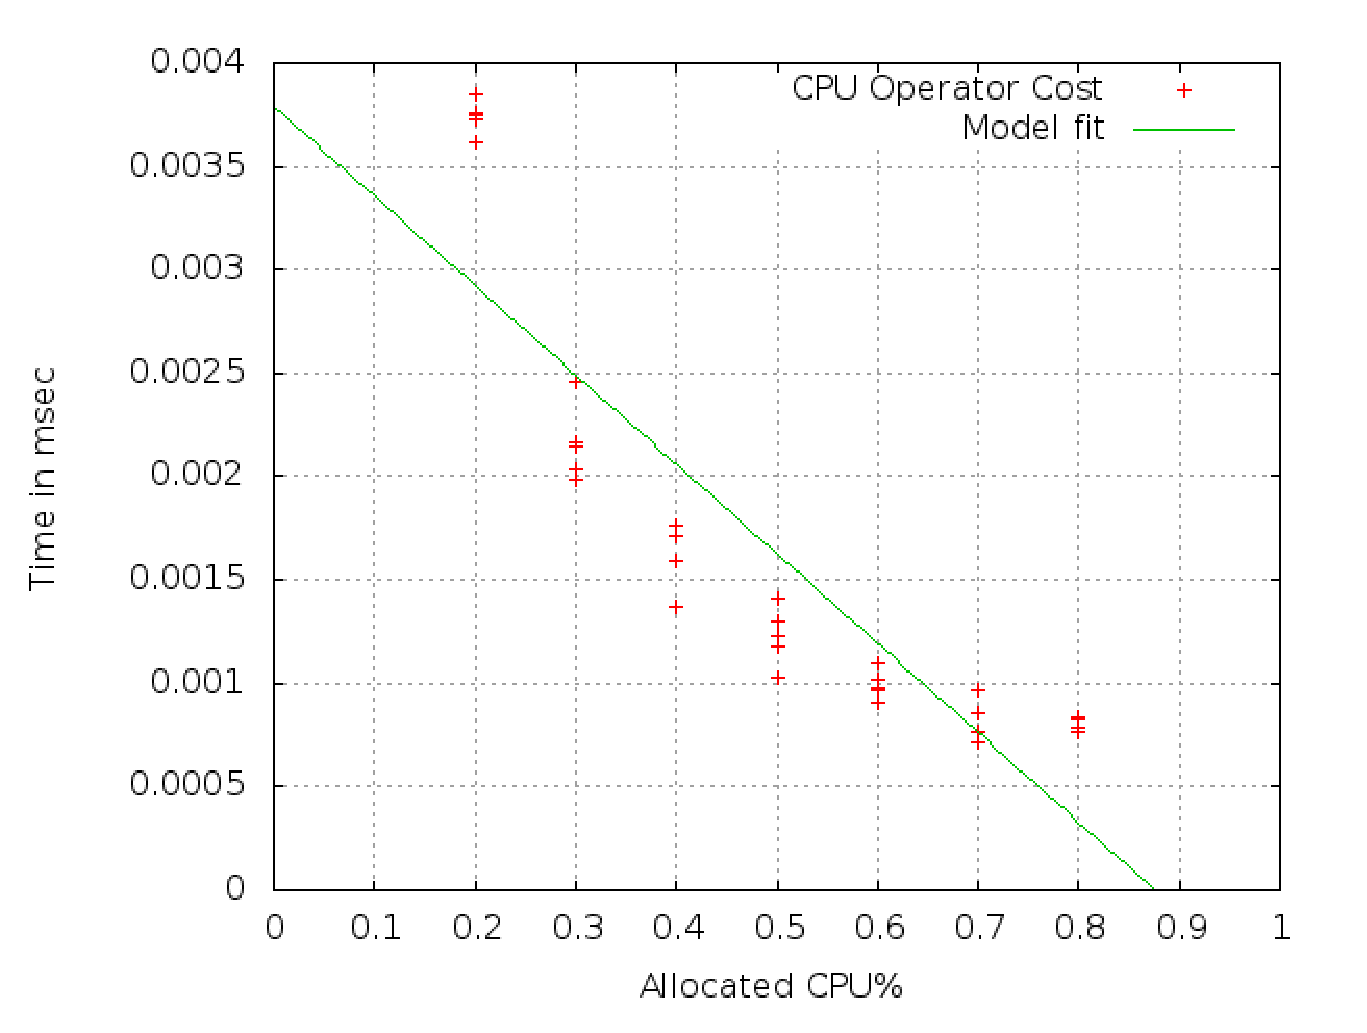
\includegraphics[width=0.5\textwidth]{cpu-operator-cost.eps}
 \caption{Mapping of the $cpu\_operator\_cost$ parameter under different resource allocation levels during calibration}
 \label{fig:cpuop}
 \end{figure} 
% 
% 
 \begin{figure}[t]
 \centering
 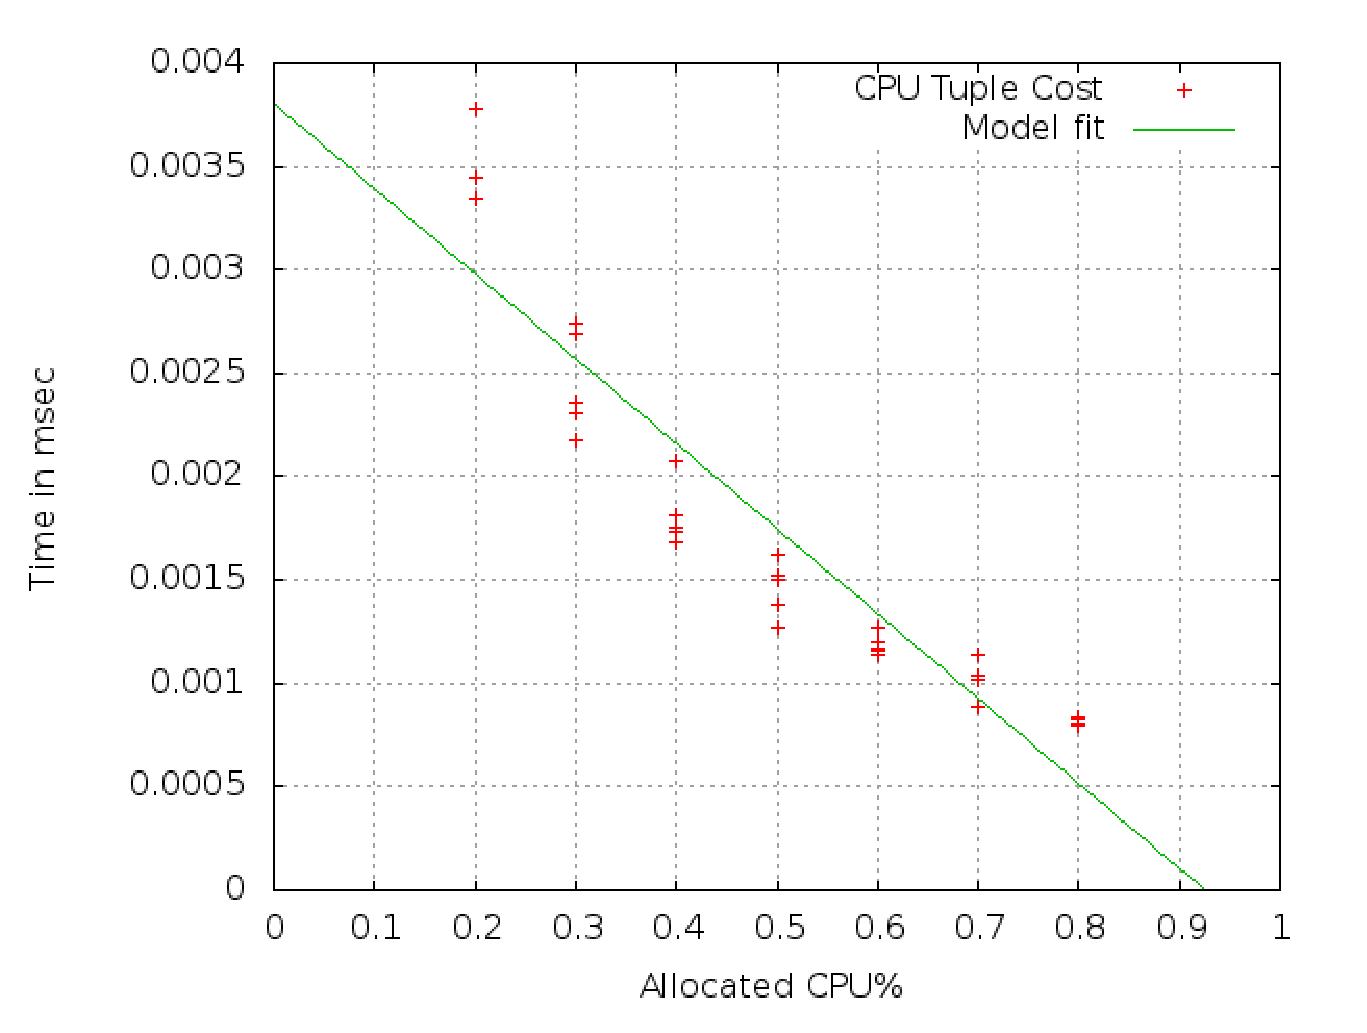
\includegraphics[width=0.5\textwidth]{cpu-tuple-cost.eps}
 \caption{Mapping of the $cpu\_tuple\_cost$ parameter under different resource allocation levels during calibration}
 \label{fig:cputp}
 \end{figure} 
 
 The calibration of the parameter \textbf{cpu\_index\_tuple} was performed according to section ~\ref{chap:implementation}. The results were obtained through the execution of the query presented in subsection ~\ref{app:cal2}. They are shown in figure ~\ref{fig:cpuip}. The errors found for linear parameters $m$ and $b$ are approximately $8.6\%$ and $5.1\%$ , respectively.

 \begin{figure}[t]
 \centering
 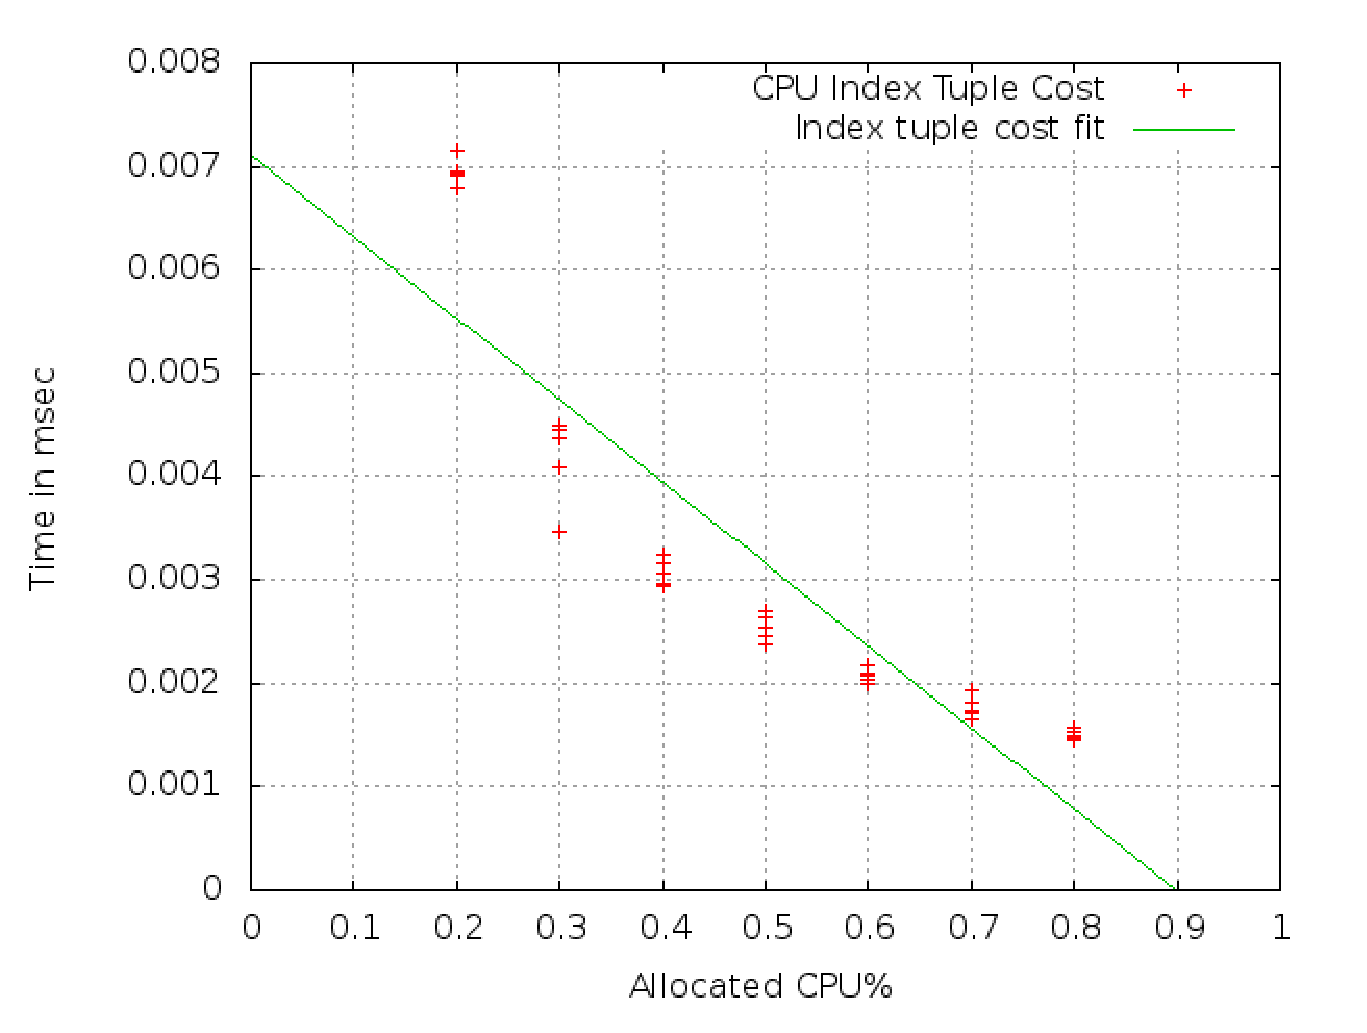
\includegraphics[width=0.5\textwidth]{cpu-index-tuple-cost.eps}
 \caption{Mapping of the $cpu\_index\_tuple\_cost$ parameter under different resource allocation levels during calibration}
 \label{fig:cpuip}
 \end{figure} 
 
\subsection{Advisor}
 

 
 To measure the performance of our advisor, we compare the costs of running the workloads under the recommended resource allocation to the default allocation. The default consists in simply allocating $1/N$ of the available CPU to the $N$ virtual machines. We consider $T_{default}$ and $T_{advisor}$ to be the execution time of the $N$ workloads running under the default resource allocation and the recommended one, respectively. The performance metric, defined in \cite{Soror:2008:AVM:1376616.1376711}, is the following:
 \[
  \frac{T_{default}-T_{advisor}}{T_{default}}
 \]
.
\subsubsection{Configuration Search}

In our first experiment, we show that the advisor can respond to different workload needs. Two TPC-H queries are used for this experiment, Q18 and Q21. In \cite{Soror:2008:AVM:1376616.1376711}, Q18 is described as one of the most CPU intensive queries. On the other hand, Q21 is one of the least CPU intensive queries, but it is much more I/O intensive than Q18. Based on these queries, two workload units are created. The first is the CPU-intensive workload unit, called C, which consists in instances of Q18. The second is the CPU non-intensive workload unit, called I, built with Q21 instances. Both of these units are scaled to have approximately the same execution time.

Based on these workload units, we create two workloads that are run by two different virtual machines. They are shown below:
\begin{eqnarray*}
 W_{1} &=& 5*C + 5*I \\
 W_{2} &=& k*C + (10-k)*I, 0 \leq k \leq 10. \\
\end{eqnarray*}
As $k$ increases, $W_{2}$ becomes more CPU intensive, while $W_{1}$ remains the same. The correct decision to be taken by our advisor as $k$ increases is to give $W_{2}$ more CPU. The results obtained are shown in figure ~\ref{fig:intensity}. For small $k$, the advisor is able to detect that $W_{2}$ is less CPU intensive, and most of the CPU allocation is given to $W_{1}$. The overall performance is improved  over the default allocation. As $k$ approaches $5$, the workloads become more alike. In this case, improvement is not possible. When $k$ is above $6$, new improvement  opportunities can be found by allocating more CPU to $W_{2}$. However the improvement is not at the same level as before, because both workloads are significantly CPU intensive. This means that the additional CPU allocation, given to $W_{2}$, causes a major performance decrease in $W_{1}$.

\begin{figure}[t]
 \centering
 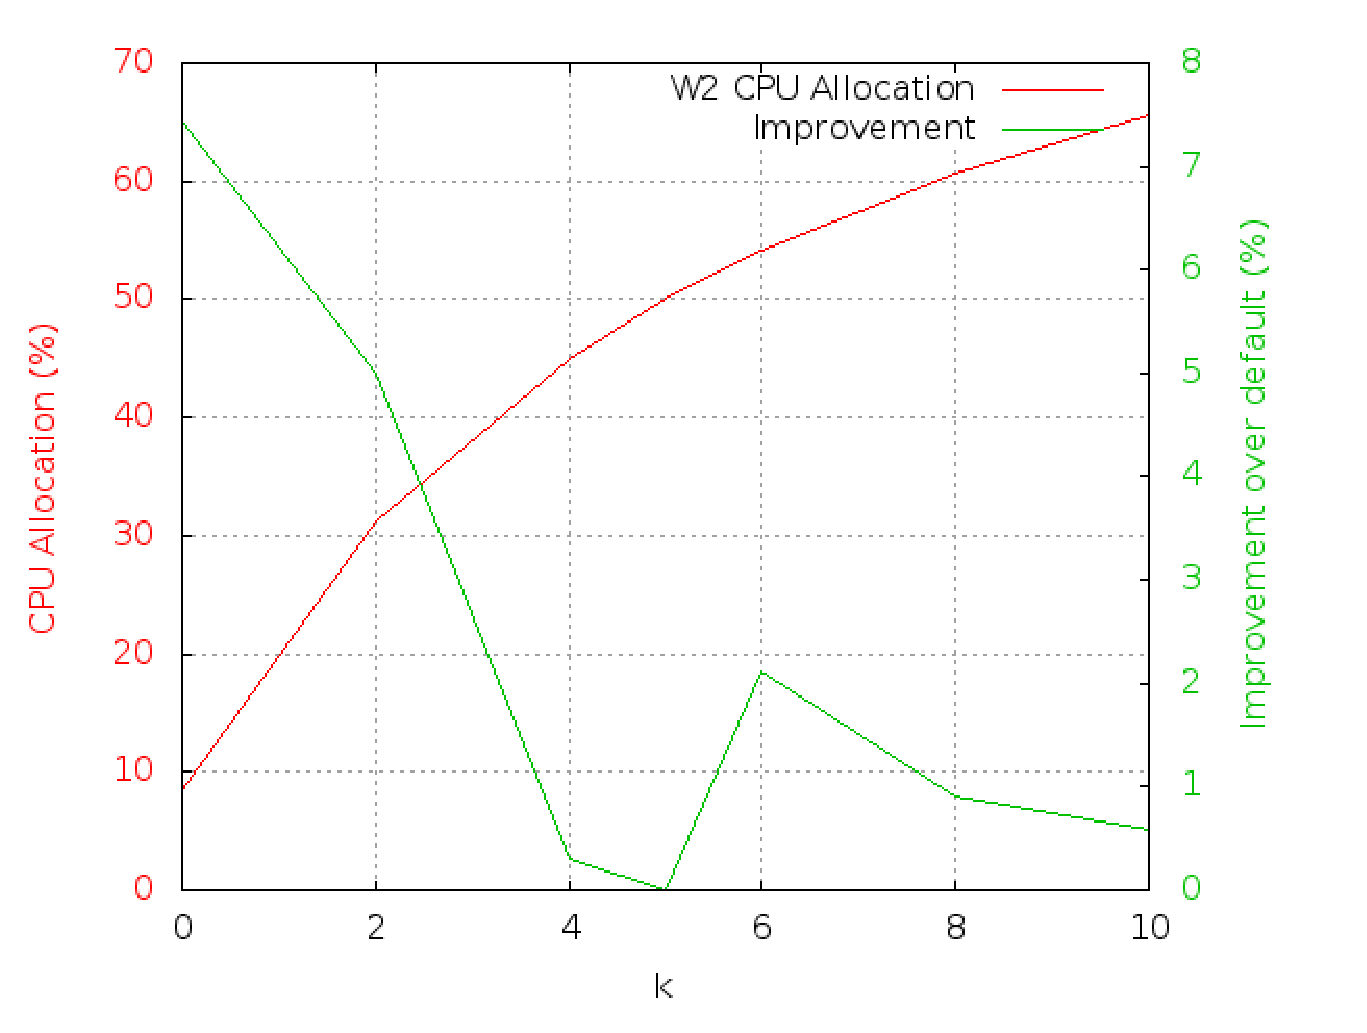
\includegraphics[width=0.5\textwidth]{improvement.eps}
 \caption{Improvement achieved through configuration search for different CPU intensity levels}
 \label{fig:intensity}
\end{figure} 

The first experiment was also performed in \cite{Soror:2008:AVM:1376616.1376711} for two DBMSes, PostgreSQL 8.1.3 and DB2\footnote{http://www-01.ibm.com/software/data/db2/} V9.  The results obtained for PostgreSQL are significantly worse than those achieved in our implementation, specially for small $k$. They are shown in figure ~\ref{fig:cpuvar-psql}. The improvement rates found in \cite{Soror:2008:AVM:1376616.1376711} are generally below $2\%$. However, they are not very clear about where the TPC-H databases are loaded ( i.e. what type of file system and hardware was used ) and whether the I/O is proportionated among VMs or not. Furthermore, since they use Xen\footnote{http://www.xen.org/} as their hypervisor, they do not specify what type of virtualization technology they use. Xen supports both paravirtualization and hardware assisted virtualization. The virtualization choice affects the performance obtained during execution, although describing how the performance is affected is out of the scope of this 
article.

\begin{figure}[t]
 \centering
 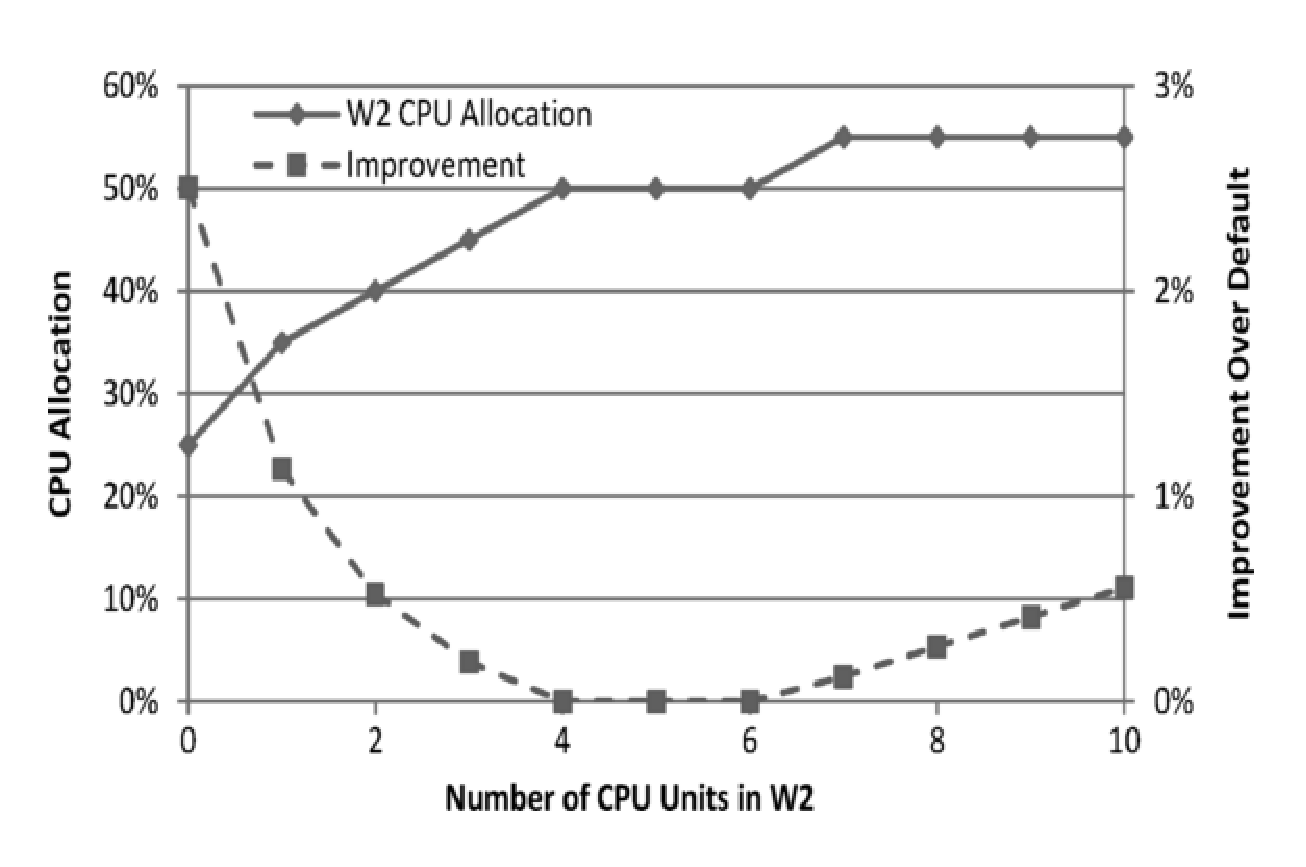
\includegraphics[width=0.45\textwidth]{CPU-var-psql.eps}
 \caption{First experiment for PostgreSQL performed in \protect\cite{Soror:2008:AVM:1376616.1376711}  }
 \label{fig:cpuvar-psql}
\end{figure} 

\subsubsection{Online Refinement}

The objective of the online refinement is to correct errors in the cost estimator model. However, it also adapts the cost model to small changes in the workload. This means that there are two ways of testing this feature. The first is to run workloads for which the DBMS cost estimator has wrong estimates about. In this case, the errors need to be known beforehand. The second way of testing it is by analyzing how the advisor behaves for small changes in the workload. Using this second approach, we adapt the workloads presented in the first experiment in a second test. Although the online refinement was not disabled in the previous experiment, the workload did not change its needs along the execution. In this second experiment, we test the online refinement feature by modifying the workload along the execution. As $k$ increases, our advisor will try to adapt the model to these changes.

In this test $W_{1}$ and $W_{2}$ are defined as follows:
\begin{eqnarray*}
 W_{1} &=& 3*C + 2*I \\
 W_{2} &=& k*C + (5-k)*I, 0 \leq k \leq 2. \\
\end{eqnarray*}

We vary $k$ from $0$ to $2$ for $W_{2}$, while $W_{1}$ remains unchanged. Instead of comparing the results of the online refinement exclusively to the default allocation, we also compare it to the case in which only the initial configuration search is enabled. This way it is possible to analyze how disabling the online refinement and maintaining static decisions about the workloads may affect the overall performance. The results are shown in figure ~\ref{fig:online-ref-pf}. There it can be seen that without the online refinement, the performance is actually decreased. This happens because $W_{2}$ is treated as a CPU non-intensive workload all the time, thus its CPU needs are underestimated.
\begin{figure}[t]
 \centering
 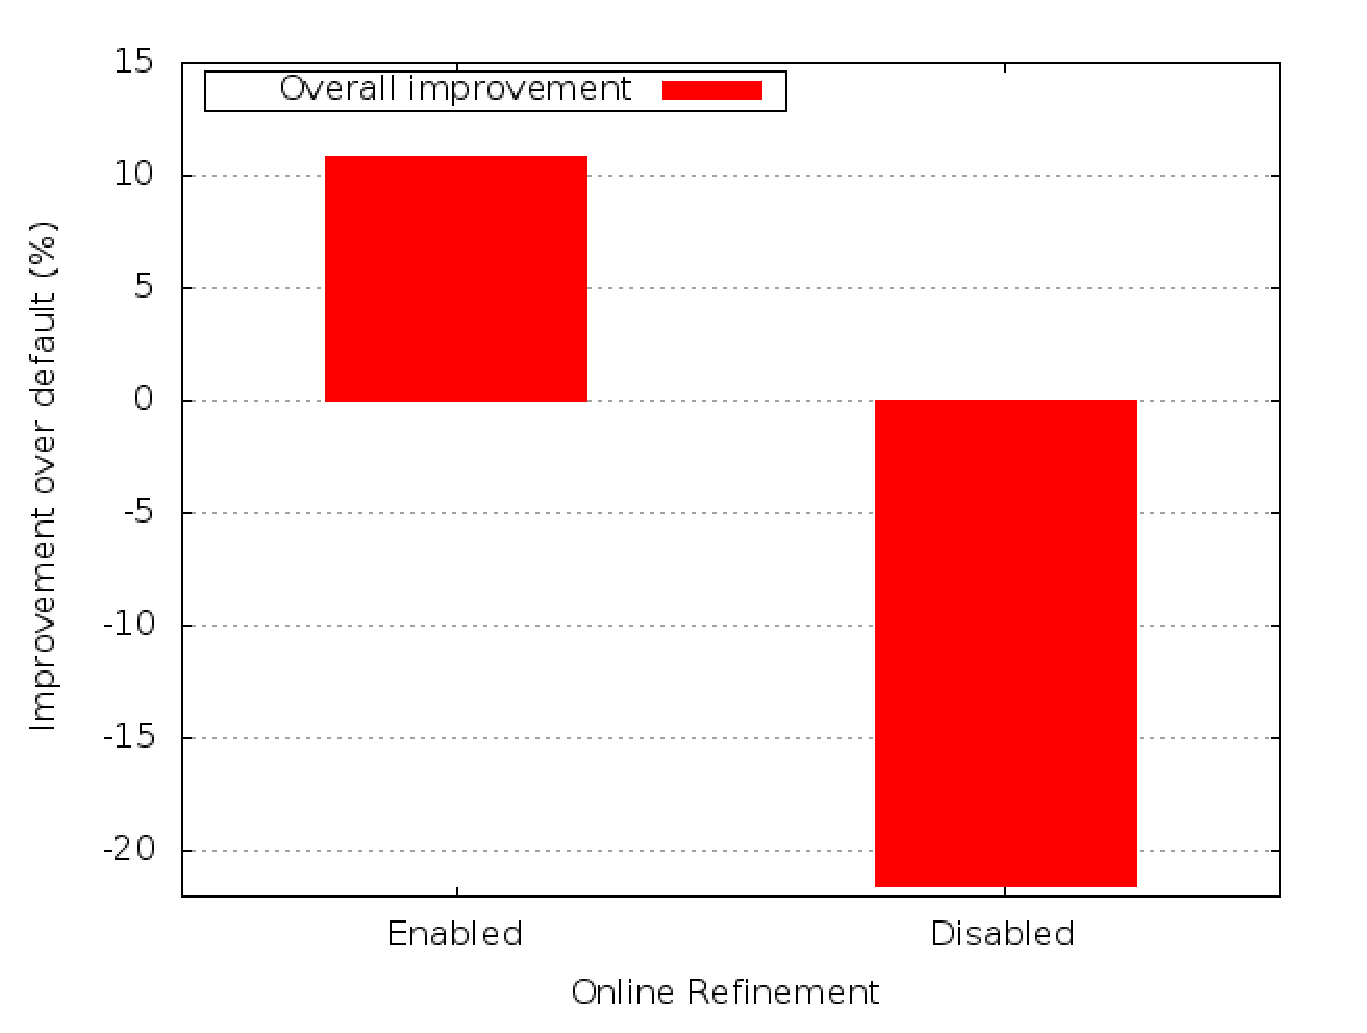
\includegraphics[width=0.5\textwidth]{online-ref.eps}
 \caption{Online refinement effects on the improvement for the second experiment}
 \label{fig:online-ref-pf}
\end{figure} 

\subsubsection{Dynamic Configuration Management}

In OpenRC, this module is responsible for detecting major changes in the workload. In order to test it, it is necessary to cause abrupt changes in the workload needs. This way we are able to see how quickly the restart of the cost model can adjust our estimates. In this test, we compare two TPC-H workloads, called $W_{3}$ and $W_{4}$. Each one of them runs in separate virtual machines. Initially, $W_{3}$ more CPU intensive than $W_{4}$. At some point in execution, these workloads have their characteristics swapped ( i.e. $W_{4}$ becomes more CPU intensive than $W_{3}$ )

This experiment is run twice. At the first time, the dynamic configuration management is disabled. This means that we rely only on the online refinement for correcting the cost model. For the second run, we enable the detection for major workload changes. Our objective is to find out how faster we are able to achieve an optimal allocation by restarting the cost model from scratch.

The advisor is set up to monitor the workloads for changes at each $960$ seconds, and it will consider changes above $20\%$ in CPU needs as major changes. The workloads are split in several units. In figure ~\ref{fig:wkchanges}, we show the CPU allocation along the workload execution organized in periods. Each period defines a moment in which the configuration search was called. The class \textbf{DynamicConfigurationManagement} checks for workload changes just before the fourth period, while the actual swap in the workload needs starts happening after the third period. Once the workloads stabilize, the workload with high CPU needs should receive approximately $70\%$  of the available CPU. Here we show that by restarting the cost model, we can converge to the optimal value faster. At the fifth step of this experiment, $W_{3}$  was still considered less CPU intensive than $W_{4}$. This would incur in a much bigger problem for workloads that change frequently.

\begin{figure}[t]
 \centering
 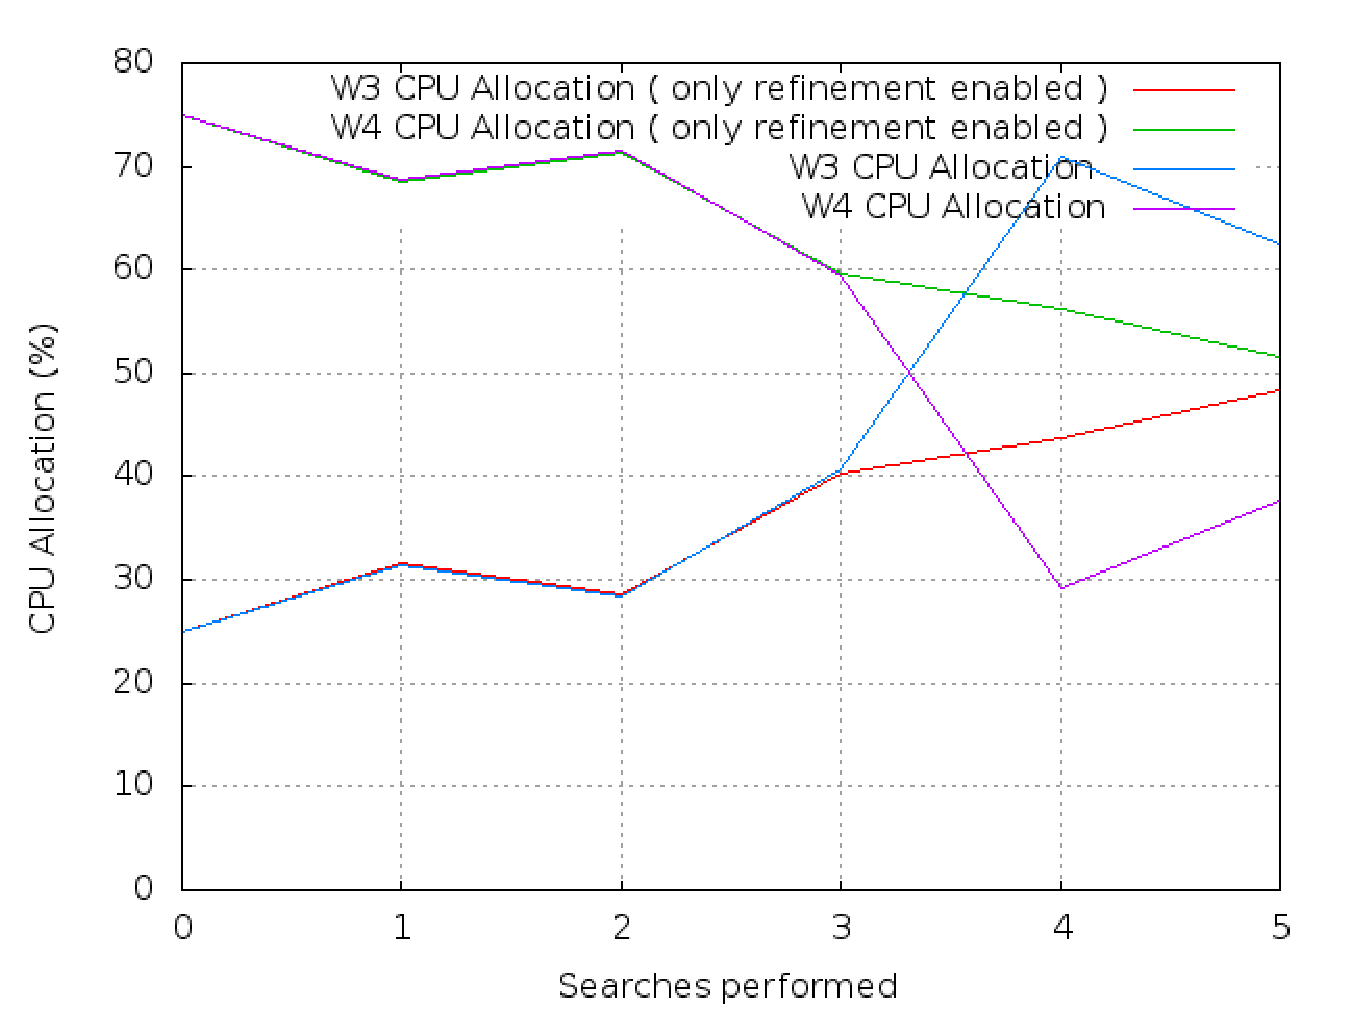
\includegraphics[width=0.5\textwidth]{dyn-change.eps}
 \caption{Dynamic configuration management effects for the third experiment}
 \label{fig:wkchanges}
\end{figure} 


\section{Final considerations}
\label{chap:final}

In this article, we aimed to solve the virtualization design problem in a private cloud. By implementing the virtualization design advisor over OpenNebula, we showed that this is possible. The advisor is responsible for improving the overall performance of running multiple database workloads in each host from the cloud. We optimize the CPU allocation among different VM guests and rely on OpenNebula for automatizing this task along the cloud.

Through experiments, we showed that we are able to identify the workload needs by leveraging the cost model built within the DBMS. We achieved a gain up to $8\%$ in initial tests. It was also possible to see that the mechanism created to dynamically correct estimative errors in the cost model works effectively. Besides propitiating a improvement of about $10\%$ over the default allocation, it also prevents the advisor from making incorrect allocation decisions, thus causing a deterioration in performance. Along with a module created to detect major changes in the workload, the advisor is able to adapt the cost models to fluctuations in the workload.


Regarding future work, there is a lot of improvement to be made in database consolidation. Obvious directions include expanding the virtualization design advisor, in order to support new resource types and DBMSes. Further experiments could show the effects of changing the workload intensity when running the workloads. Furthermore, the cloud infrastructure could be more exploited. For instance, VM migration could be used to transfer VMs to hosts with more available resources.  This feature is already supported by OpenNebula. The problem is how to optimize these transfers, because they generate a high overhead. 


%%%%%%%%%%%%%%%%%%%%%%%%%%%%%%%%%%%%%%%%%%%%%%%%%%%%%%%%%%%%%%%%%%%%%%%%%%%%%%%%%%%%%%%%%%%%%%%
\appendix
%%%%%%%%%%%%%%%%%%%%%%%%%%%%%%%%%%%%%%%%%%%%%%%%%%%%%%%%%%%%%%%%%%%%%%%%%%%%%%%%%%%%%%%%%%%%%%%


\section{CPU allocation decision algorithm}
\label{sec:cpusearch}

\begin{algorithm}[H]
 \begin{algorithmic}
    \FOR{$i = 1 \to N$} 
	\STATE $r_{i} \gets \frac{1}{N}$
    \ENDFOR
    
    \STATE $ Sum_{i} \gets 0 $
    \FOR{$i = 1 \to N$}
	\STATE \COMMENT{Find out how much $W_{i}$ benefits from adjusting the resource }

	\STATE $ Slope_{i} \gets Cost(W_{i},r_{i}) - Cost(W_{i},r_{i} + \delta)$
	\STATE $ Sum_{i} \gets Sum_{i} + Slope_{i} $
    \ENDFOR
    \FOR{$i = 1 \to N$}
	\STATE \COMMENT{ Set the appropriate CPU allocation level of $W_{i}$. Ratio is the relative improvement of $W_{i}$ }
	\STATE $ Ratio_{i} \gets Slope_{i} * Sum_{i} $
	\STATE $ R_{i} \gets N*Ratio_{i} $
    \ENDFOR

 \end{algorithmic}
  \caption{Greedy search algorithm}
  %\label{alg:greedy}
\end{algorithm}

\section{Calibration queries}

\subsection{cpu\_tuple\_cost and cpu\_operator\_cost}
\label{app:cal1}
\lstinputlisting{../../queries/aggregate-seq-scan.sql}

\subsection{cpu\_index\_tuple\_cost}
\label{app:cal2}
\lstinputlisting{../../queries/index-scan.sql}

	
% INCLUDE BIBLIOGRAPHY WHICH MUST FOLLOW jidm.bst TEMPLATE
\bibliographystyle{jidm}
\bibliography{jidmb}
% For information on how to write bibliography entries, 
% see file jidmb.bib

\begin{received}
\end{received}

\end{document}
